\documentclass [11pt,twoside]{article}
\usepackage[utf8]{inputenc}
\usepackage[T1]{fontenc}
% to add numbers to paragraphs
\usepackage{titlesec}
% for verbatim text input
\usepackage{fancyvrb}

% to add numbers to paragraphs
\setcounter{secnumdepth}{4}

%Page margins, header and footer positions
\usepackage{geometry}
 \geometry{
 a4paper,
 total={210mm,297mm},
 left=25mm,
 right=25mm,
 top=30mm,
 bottom=25mm,
 headsep=7mm}

\interfootnotelinepenalty=10000

%To display filling dots in the TOC for all entries
\usepackage[titles]{tocloft}
\renewcommand{\cftsecleader}{\cftdotfill{\cftdotsep}}

%Define new header and footer style
\usepackage{fancyhdr}

\pagestyle{fancy}
\fancyhf{}
\lhead{\color{Gray}{\small{CLup project by Simone Abelli, Stefano Azzone}}}
\lfoot{\textcolor{Gray}{\small{Copyright © 2017, Simone Abelli, Stefano Azzone – All rights reserved}}}
\rfoot{\textcolor{Gray}{\thepage}}
\renewcommand{\headrulewidth}{0pt}

%PACKAGES
\usepackage{wasysym}
\usepackage{pifont}

\newcommand{\supported}{\ding{52}\xspace}
\newcommand{\unsupported}{\ding{55}\xspace}
\newcommand{\partsupported}{\textcolor{black!40}{\ding{52}}\xspace}
\newcommand{\lowsupported}{\textcolor{black!20}{\ding{52}}\xspace}
\newcommand{\unknowsupported}{\textbf{?}\xspace}

%Font: Times
\usepackage{times}
%Change monospaced font
\renewcommand{\ttdefault}{lmtt}

%tables
\usepackage{tabu}
\usepackage{tabularx}
\usepackage{ltablex}
\usepackage{longtable}
\usepackage{float} % To allow the use of H modifier in long tables

%landscape mode
\usepackage{pdflscape}
\usepackage{rotating}
\usepackage{caption}

%make landscape mode be sensitive to even and odd pages
%start
\def\myrotate{\ifodd\c@page\else-\fi 90}
\makeatletter
\global\let\orig@begin@landscape=\landscape%
\global\let\orig@end@landscape=\endlandscape%
\gdef\@true{1}
\gdef\@false{0}
\gdef\landscape{%
    \global\let\within@landscape=\@true%
    \orig@begin@landscape%
}%
\gdef\endlandscape{%
    \orig@end@landscape%
    \global\let\within@landscape=\@false%
}%
\@ifpackageloaded{pdflscape}{%
    \gdef\pdf@landscape@rotate{\PLS@Rotate}%
}{
    \gdef\pdf@landscape@rotate#1{}%
}
\let\latex@outputpage\@outputpage
\def\@outputpage{
    \ifx\within@landscape\@true%
        \if@twoside%
            \ifodd\c@page%
                \gdef\LS@rot{\setbox\@outputbox\vbox{%
                    \pdf@landscape@rotate{-90}%
                    \hbox{\rotatebox{90}{\hbox{\rotatebox{180}{\box\@outputbox}}}}}%
                }%
            \else%
                \gdef\LS@rot{\setbox\@outputbox\vbox{%
                    \pdf@landscape@rotate{+90}%
                    \hbox{\rotatebox{90}{\hbox{\rotatebox{0}{\box\@outputbox}}}}}%
                }%
            \fi%
        \else%
            \gdef\LS@rot{\setbox\@outputbox\vbox{%
                \pdf@landscape@rotate{+90}%
                \hbox{\rotatebox{90}{\hbox{\rotatebox{0}{\box\@outputbox}}}}}%
            }%
        \fi%
    \fi%
    \latex@outputpage%
}
\makeatother
%end

%graphics
\usepackage{graphicx}
\usepackage[dvipsnames, table]{xcolor}
%If you upload images from PC, you need to insert code for the path here (different for Windows and Unix OS)

%References
%\usepackage{xpatch}
%\usepackage[backend=biber, style=numeric, citestyle=numeric, sorting=none]{biblatex}
%\addbibresource{main.bib}

%Other
\usepackage{ifthen}
\usepackage{xspace}
\usepackage{enumitem}
\usepackage{amssymb}
\usepackage[pdftex, colorlinks]{hyperref}
\newcommand{\comment}[1]{{\color{Red}$\blacktriangleright$ Comment: #1 $\blacktriangleleft$}}


% Some utilities\ldots
\usepackage{soul}
\usepackage{tikz}

\usetikzlibrary{calc}
\usetikzlibrary{decorations.pathmorphing}


\makeatletter

\newcommand{\defhighlighter}[3][]{%
  \tikzset{every highlighter/.style={color=#2, fill opacity=#3, #1}}%
}

\defhighlighter{yellow}{.5}

\newcommand{\highlight@DoHighlight}{
  \fill [ decoration = {random steps, amplitude=1pt, segment length=15pt}
        , outer sep = -15pt, inner sep = 0pt, decorate
       , every highlighter, this highlighter ]
        ($(begin highlight)+(0,8pt)$) rectangle ($(end highlight)+(0,-3pt)$) ;
}

\newcommand{\highlight@BeginHighlight}{
  \coordinate (begin highlight) at (0,0) ;
}

\newcommand{\highlight@EndHighlight}{
  \coordinate (end highlight) at (0,0) ;
}

\newdimen\highlight@previous
\newdimen\highlight@current

\DeclareRobustCommand*\highlight[1][]{%
  \tikzset{this highlighter/.style={#1}}%
  \SOUL@setup
  %
  \def\SOUL@preamble{%
    \begin{tikzpicture}[overlay, remember picture]
      \highlight@BeginHighlight
      \highlight@EndHighlight
    \end{tikzpicture}%
  }%
  %
  \def\SOUL@postamble{%
    \begin{tikzpicture}[overlay, remember picture]
      \highlight@EndHighlight
      \highlight@DoHighlight
    \end{tikzpicture}%
  }%
  %
  \def\SOUL@everyhyphen{%
    \discretionary{%
      \SOUL@setkern\SOUL@hyphkern
      \SOUL@sethyphenchar
      \tikz[overlay, remember picture] \highlight@EndHighlight ;%
    }{%
    }{%
      \SOUL@setkern\SOUL@charkern
    }%
  }%
  %
  \def\SOUL@everyexhyphen##1{%
    \SOUL@setkern\SOUL@hyphkern
    \hbox{##1}%
    \discretionary{%
      \tikz[overlay, remember picture] \highlight@EndHighlight ;%
    }{%
    }{%
      \SOUL@setkern\SOUL@charkern
    }%
  }%
  %
  \def\SOUL@everysyllable{%
    \begin{tikzpicture}[overlay, remember picture]
      \path let \p0 = (begin highlight), \p1 = (0,0) in \pgfextra
        \global\highlight@previous=\y0
        \global\highlight@current =\y1
      \endpgfextra (0,0) ;
      \ifdim\highlight@current < \highlight@previous
        \highlight@DoHighlight
        \highlight@BeginHighlight
      \fi
    \end{tikzpicture}%
    \the\SOUL@syllable
    \tikz[overlay, remember picture] \highlight@EndHighlight ;%
  }%
  \SOUL@
}

\makeatother

% Common abbrev. are set as commands to ensure proper spacing after the dot
\RequirePackage{xspace}
\newcommand{\ie}{i.e.\@\xspace}
\newcommand{\aka}{a.k.a.\@\xspace}
\newcommand{\Ie}{I.e.\@\xspace}
\newcommand{\cf}{cf.\@\xspace}
\newcommand{\Cf}{Cf.\@\xspace}
\newcommand{\eg}{e.g.\@\xspace}
\newcommand{\Eg}{E.g.\@\xspace}
\newcommand{\etal}{et al.\@\xspace}
\newcommand{\etc}{etc.\@\xspace}
\newcommand{\wrt}{w.r.t.\@\xspace}
\newcommand{\Wrt}{W.r.t.\@\xspace}



\date{}

\usepackage[utf8]{inputenc}
\usepackage[dvipsnames]{xcolor}
\usepackage{listings}
\usepackage{alloy-style}
\begin{document}

%TITLE PAGE

\begin{titlepage}


%LOGO

\centering

\includegraphics[scale=0.5]{Images/PolimiLogo}

\vspace{4cm}
%TITLE 

{\textcolor{Blue}{\textbf{\Huge{CLup}}}} \\ [1cm]


\vspace{4cm}

%Replace the text string with your title
{\textcolor{Blue}{\textbf{\Huge{Requirement Analysis and Specification
        Document}}}} \\ [1cm]

\vspace{4cm}
Simone Abelli \\
Stefano Azzone

\end{titlepage}

%Define deliverable specific info
%Replace cell contents where needed
\begin{table}[h!]
\begin{tabu} to \textwidth { X[0.3,r,p] X[0.7,l,p] }
\hline

\textbf{Deliverable:} & RASD\\
\textbf{Title:} & Requirement Analysis and Verification Document \\
\textbf{Authors:} & Simone Abelli, Stefano Azzone \\
\textbf{Version:} & 1.0 \\ 
\textbf{Date:} & 7 November 2016 \\
\textbf{Download page:} & https://github.com/StefanoAzzone/AbelliAzzone \\
\textbf{Copyright:} & Copyright © 2017, Simone Abelli, Stefano Azzone – All rights reserved \\
\hline
\end{tabu}
\end{table}




\setcounter{page}{2}


%------------------------------------------------------------------------------------------------------------------------------------------------
\newpage

\tableofcontents


%------------------------------------------------------------------------------------------------------------------------------------------------
\clearpage
{\color{Blue}{\section{Introduction}}}
\label{sect:introduction}
\subsection{Purpose}
The coronavirus emergency has put a strain on society on many levels, in  particular,  grocery  shopping can  become  a  challenge  in  the presence  of  such  strict  rules: supermarkets  need to  restrict  access  to  their  stores  to  avoid having  crowds  inside and long  lines outside. The  goal  of  this  project  is  to  develop  an  easy-to-use  application  that,  on  the  one  side,  allows  store managers  to  regulate  the  influx  of  people  in  the  building  and,  on  the  other  side,  saves  people  from having to line up and stand outside of stores for hours on end. \\\\
The application will allow customers to “line up” (i.e., retrieve a number) from their home, and then wait  until  their  number  is  called  (or  is  close  to  being  called)  to  approach  the  store.  In  addition,  the application could be used to generate QR codes that would be scanned upon entering the store, thus allowing store managers to monitor entrances.\\\\
The system must attain the following goals:

\begin{enumerate}[label=G\arabic*]
	\item CLup should allow customers to queue up remotely and on premise in such a way that they don't need to form a physical line
	\item CLup should allow store owners to regulate how many customers can be simultaneously in their stores
	\item CLup should provide the customer with a reasonably precise estimate of waiting time
	\item CLup should alert the customers when it is time to get to the shop taking into account travel time
	\item CLup should allow customers to book future visits to stores
	%\item CLup should allow customers to specify estimated visit duration and desired objects in order to provide a better guess of waiting time for all the customers
	%TODO is this a goal or a reqirement???
	\item CLup should be able to infer an approximate duration of the visit from an analysis of the previous ones to plan visits and manage the queue in a finer way
\end{enumerate}


%Identify product and application domain
%analysis of the world and of the shared phenomena
\subsection{Scope}
The system to be allows to avoid creating queues in front of stores.
This is accomplished by enabling the customers to queue up remotely.
Moreover, the shop owners can oversee customers entering and exiting stores. \\
The system offers the following functionalities:
%TODO: they look a lot like goals/product functions, substitute with (slides):
% Identifies the product and 
% application domain
\begin{enumerate}[label=F\arabic*]
	\item it allows customers to line up remotely or on premise
	\item it allows customers whose position in queue allows it to enter and exit the store
	\item it schedules customers in order to minimize overcrowding inside and outside of the store
	\item it alerts customers when they should head to the store
	\item it allows customers to book a visit and optionally specify duration and desired categories of products
	\item it allows store owners to monitor flux of people inside the store and set how many customers can be simultaneously inside
	\item it allows store owners to register stores
	\item it uses statistics build on entrance and exit data, and preferred categories to better evaluate duration of visits
\end{enumerate}
User can access the system using a phone application provided that they own a smartphone with an internet connection. This application allows registered users to easily access the functionality of the system.\\Moreover, for those who do not have access to the required technology or don't want to use the phone application, there is also a web app. Therefore, users will be able to log in and perform the same operations of the phone application using an internet browser.\\ Finally the customers of the store will also have the possibility to create reservations on premise: every shop will be equipped with a device to print tickets in order to give every client a very easy way to line up. Of course customers that wants to queue up "on the spot" must have a means of identification (e.g. document), in order to prevent fake reservations that would slow down the queue. For the same reason users that use the phone application or the web app must log in to identify themselves.\\
Only customer with a valid reservation (i.e it is their turn) will be allowed to enter the store; to achieve this, each store must have a device (e.g. a QR/NFC reader) to every entrance, and clients must validate their reservation before being admitted inside. They should also do the same to exit, in order to monitor the store's occupation.
\subsubsection{World Phenomena}
\begin{enumerate}[label=WP\arabic*]
	\item Customer reaches a store
	\item Customer enters or exits a store
	\item Store owner controls current number of customers in one of his stores
	\item Customer buys products
\end{enumerate}
\subsubsection{Shared Phenomena}
\begin{enumerate}[label=SP\arabic*]
	\item Customer queues up
	\item Customer is identified %in order to allow entrance or exit from a store
	\item Turnstiles lock and unlock
	\item Customer is alerted% when his turn is close
	\item Customer books a visit to a store
	\item Printer prints a ticket
\end{enumerate}
\subsection{Definitions, Acronyms, Abbreviations}
\subsubsection{Definitions}
\begin{tabular}{ | m{5cm} | m{10cm} | }
	\hline
	Reservation & Virtual or physical artifact used to identify the position of a customer in a queue \\
	\hline
	Reservation & A place in the queue\\
	\hline
	Enqueued & A customer is enqueued when he has provided the system with a means of identification and requested a reservation\\
	\hline
	Authorized & A customer is authorized when he has been enqueued and is allowed temporary access to the store.\\
	\hline
	Occupation & Number of customers currently present in the store\\
	\hline
\end{tabular}
\subsubsection{Acronyms}
\begin{tabular}{ | m{5cm} | m{10cm} | }
	\hline
	RASD & Requirement Analysis and Specification Document \\
	\hline
	GPS & Global Positioning System \\
	\hline
	S2B & Software to be \\
	\hline
	UI & User Interface\\
	\hline
\end{tabular}
\subsubsection{Abbreviations}
\begin{tabular}{ | m{5cm} | m{10cm} | }
	\hline
	Gn & Goal number n \\
	\hline
	Rn & Requirement number n \\
	\hline
	Dn & Domain Assumption number n \\
	\hline
	WPn & World Phenomenon number n \\
	\hline
	SPn & Shared Phenomenon number n \\
	\hline
\end{tabular}
\subsection{Revision history}
Not yet defined.
\subsection{Reference Documents}
\begin{enumerate}
	\item IEEE Std 830-1998 Recommended Practice for Software Requirements Specifications
	\item Specification Document: R\&DD Assignment A.Y. 2020/2021
\end{enumerate}
\subsection{Document Structure}
\begin{itemize}
	\item Chapter 1: gives an introduction about the project, describing the purpose of the    system informally and defining its scope, its main goals, world and shared phenomena. Moreover this section contains specifications such as the definitions, acronyms, abbreviation,	revision history of the document and the references.
	\item Chapter 2: contains the overall description of the project, with a more in-depth look at its functionalities. Here are identified the main actors involved in the application’s usage lifecycle, some scenarios that point out the major features of the S2B, and all the necessary domain assumptions, dependencies and constraints. This section also provides a class diagram, which aid to better understand the general structure of the project, and some state diagrams, to make the evolution of the crucial objects clear.
	\item Chapter 3: This section contains the core of the document: first it presents the interface requirement including user, hardware, software and communication interfaces.
	Then it offers the specification and the description of all the functional requirements necessary in order to reach the goals; is also provided a list of use cases, with their corresponding sequence diagrams and their mapping on the requirements, as long as some scenarios, useful to identify specific cases in which the application can be utilized.
	Finally non-functional requirements are defined, including performance, design and the software systems attributes.
	\item Chapter 4: includes the alloy code and the corresponding metamodels generated from it, in order to show how the project has been modeled and represented through the language.   
	\item Chapter 5: shows the effort which each member of the group spent working on the project.
	\item Chapter 6: includes the reference documents.
\end{itemize}



%------------------------------------------------------------------------------------------------------------------------------------------------
\clearpage
{\color{Blue}{\section{Overall Description}}}
\label{sect:overview}
\subsection{Product perspective}
The S2B will be used by two kinds of users: customers and store owners. The system will provide customers with a simple UI, in order to be accessible for all demographics. To use the software the customers need either a smartphone or a computer (a printer may be required in this case to print a QR code on paper) with a working internet connection. The software will use a location API (e.g. Google Maps) to pinpoint the location of the customers. To allow on premise reservations the store must install a monitor and a ticket printer outside of the store, and connect them to the system.\\
The system offers to each of the users different functionalities:
\subsubsection{Customer}
The customer can create reservations for a desired store: such reservation is then inserted into a queue. This queue is managed in order to avoid overcrowding, and to serve customers with a first come first served policy (FIFO queue). To achieve this, statistics about visits' durations are exploited, taking also into account information that customers may provide (e.g. which department of the store they want to visit).\\
There are multiple types of reservations that can be requested:
\begin{enumerate}
	\item Immediate reservation: the costumer wants to queue up immediately to a store. He/she is also provided with an estimation of the time he has to wait before his/her turn.
	\item Future reservation: the costumer wants to book a future visit at a desired time and store.\\ When creating the reservation the customer can specify how long he/she intends to stay and which departments of the market he/she plans to go to, in order to provide a better plan. If he/she does not specify the duration the system can infer it using some statistic built on his/her previous visits. Then the customer will be provided whit the actual time he will be able to access the store (considering the bookings from other customers).
	\item On premise reservation: the customer is allowed to enqueue directly at the store. Each of them will provide a system to print tickets so that those who do not have access to the required technology for the previous options can still line up. These tickets contain a reservation number and an estimation of the waiting time before being able to enter.
\end{enumerate}
Each customer will be assigned a number that represents his/her position in queue. A monitor outside the store will display the number of the last customer allowed to enter.
Customers who requested an immediate or a future reservation can receive an alert when they need to depart to reach the store through their smartphone app.
This alert is based on the location of the customer, so that the time needed to reach the store is taken into account. If, for any reason, a customer cannot to go to a store he/she has lined up to it is possible for him/her to delete the immediate or future reservation. The on premise reservation cannot be deleted.\\\\
Reservations can be in one of the following states:
\begin{itemize}
	\item Pending: customer cannot yet access the store
	\item Authorized: customer can access the store
	\item Current: customer is in the store
	\item Expired: customer has exited the store or the reservation has been canceled
\end{itemize} 
\subsubsection{Store owner}
The store owner can
\begin{enumerate}
	\item Register a store to the system so that it can be accessed by customers
	\item Set the maximum occupation threshold for each of his stores.
	\item Monitor the number of customers inside at any time
	\item Visualize statistics about the flow of clients and department occupation
\end{enumerate}
When setting the maximum occupation of a store, the owner can specify a threshold for each department or for the whole store. In the latter case the occupation of each department is set to the same value. In case customers select which sections of the store they intend to visit their presence will be considered only in those specific departments, in order to allow more customers in, provided that they will not come in contact with each other. For safety, if customers don't specify anything they are supposed to visit each department.
\begin{figure}[!htb]
\centering
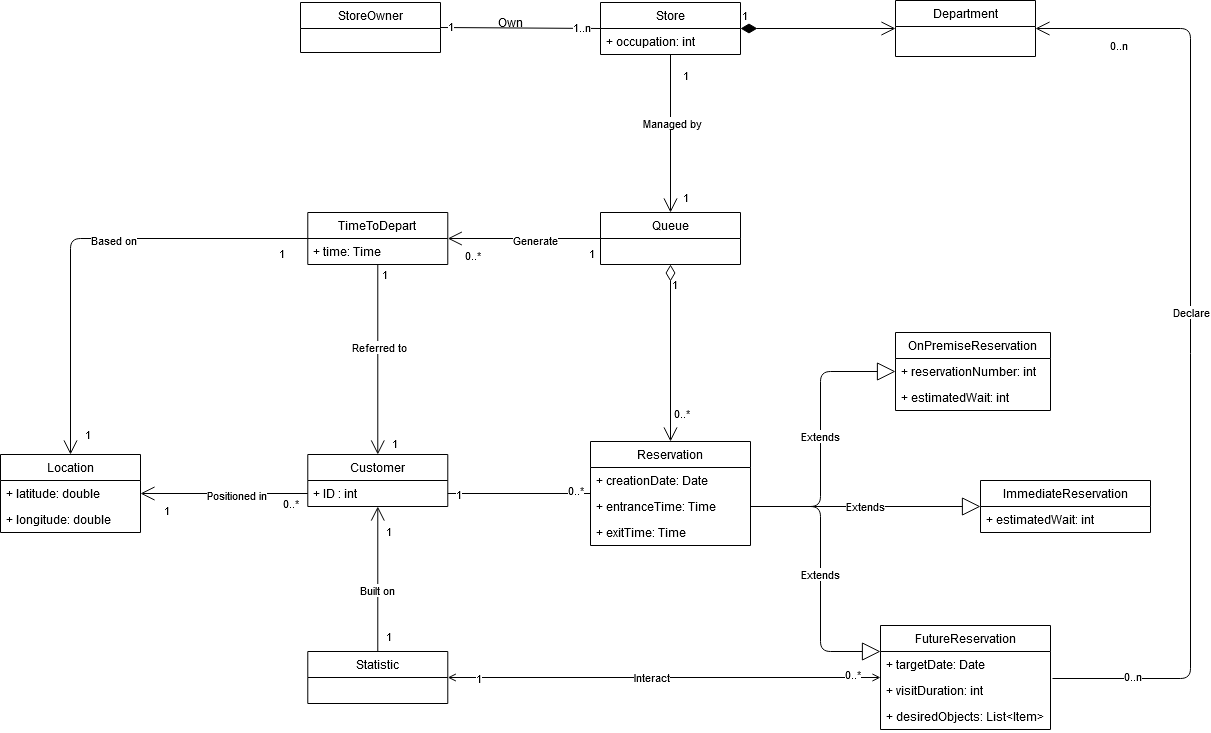
\includegraphics[width=\textwidth]{Images/ClassDiagram.png}
\caption{\label{fig:metamodel2}Class Diagram.}
\end{figure}
\newpage
\subsubsection{State charts}
Here we show the main processes that the system will manage, and the states in which the system will find itself.
\begin{figure}[!htb]
	\centering
	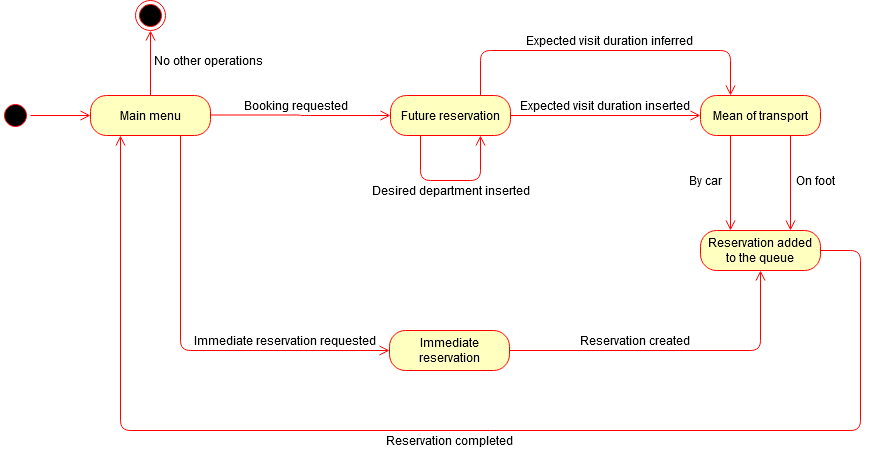
\includegraphics[width=\textwidth]{Images/StateDiagram1.png}
	\caption{\label{fig:metamodel3}State Diagram 1: Creation of a reservation.}
\end{figure}\\
%TODO add by car/on foot request
The figure above illustrates how the customer creates a reservation (virtual customer). The customer accesses the main menu. From there he/she can request an immediate reservation or a future reservation. If he/she requests an immediate reservation, it is created and the process terminates. If he/she requires a future reservation he can add the departments he/she intends to visit, and how much time he/she is going to spend at the store. Then the reservation is created and the process terminates.\\\\\\\\

\begin{figure}[!htb]
	\centering
	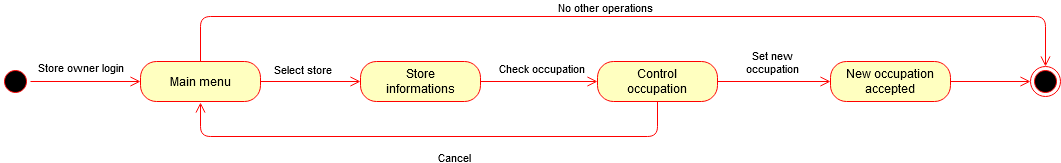
\includegraphics[width=\textwidth]{Images/StateDiagram2.png}
	\caption{State Diagram 2: Store owner sets occupation.}
\end{figure}
The figure above illustrates how the store owner sets the maximum occupation of one of his stores. The store owner logs in and is provided a main menu. He/she selects one of his stores, and is presented with the current maximum occupation of his selected store. He can change it to a value to his liking, or go back to the main menu.
\newpage

\begin{figure}[!htb]
	\centering
	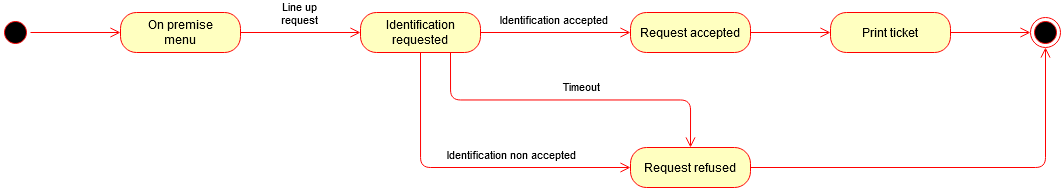
\includegraphics[width=\textwidth]{Images/StateDiagram3.png}
	\caption{State Diagram 3: On premise creation of a reservation.}
\end{figure}
The figure above illustrates how a customer can queue up on premise (physical customer). The customer is presented with an on premise main menu. From there he/she can request to queue up (create a reservation) immediately. He will be prompted to identify himself (e.g. social security card). Once identified the customer will be provided a ticket with a number that represents his position in queue and an estimate of the waiting time.

\begin{figure}[!htb]
	\centering
	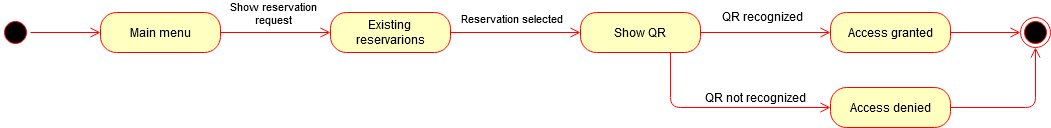
\includegraphics[width=\textwidth]{Images/StateDiagram4.png}
	\caption{State Diagram 3: Customer enters a store.}
\end{figure}
The figure above illustrates how a customer who is authorized can access the store. At the entrance of his/her store of choice he is enabled to demonstrate his authorization. Once he/she does, he is allowed to enter the store.

\subsubsection{Scenarios}
\paragraph{Customer queues up remotely}
Gordon comes home from work at 5:30 PM. He would like to go to the store. He is a registered user of CLup. His smartphone has internet connection and GPS on. He opens the CLup mobile application and requests an immediate reservation to a store of his choice, selecting the car as means of transport. After some time he is alerted that he needs to depart to avoid being late at the store and losing the reservation. Gordon departs and arrives to the store. He opens the application and selects the reservation he created which now contains the number that represents his position in the queue. After some time the monitor outside the store shows his number, which means it is his turn to enter. He activates the turnstiles with the QR now shown in the reservation page of the mobile application and enters the store. He buys all the products he needs. He opens the application and selects the reservation he created which now contains a QR code. He activates the turnstiles and exits the store.
\paragraph{Customer queues up on premise}
Marco is an old man. He does not have a smartphone. He would like to go to the store next to his house on foot. He reaches the store, and retrieves a queue reservation ticket from the printer outside the store, by inserting his social security card. The ticket displays a QR code, a number that represents his position in queue and an estimated waiting time. He can now come back home and wait the specified amount of time, then come back to the store. At that point the monitor outside the store shows his number, which means it is his turn to enter. He activates the turnstiles with the QR printed on his ticket and enters the store. He buys all the products he needs. He activates the turnstiles with his ticket and exits the store.
\paragraph{Store owner registering a store and setting occupation}
Paolo is the proud owner of the famous supermarket chain "Junes" and today there is the first opening of a new store of the chain. Due to Covid restrictions, he already use CLup to avoid overcrowding inside his stores. He decide to use the service also for the new building, so he access the system through his PC. Once logged in he register his new supermarket by inserting all necessary data. Then he select the newly registered store and set an appropriate occupation for each of its department, based on how many people it can contain, ensuring social distances.
\paragraph{Customer books a visit}
Lara is very organized woman; she likes to manage situations in advance, and for this reason, in the recent period, she uses CLup to book her visit to the store. Every Sunday she open the CLup web page from her phone, logs in and create a new reservation for the next Saturday. Because she request this reservations in advance af almost a week, she usually has no problems to book exactly for the time she prefer, so she is able to get an appointment for the 9.30 and print the ticket. In this way when the time arrives she can enter the store with no delays and rows.

\subsection{Product functions}
We describe here functions that the system will support.
\begin{enumerate}
	\item Customers can queue up virtually or physically, immediately or in the future at one of the stores registered to the service.
	\item Customers can delete a virtual reservation.
	\item Customers can access the desired store when its occupation reaches acceptable levels.
	\item Customers that queued up virtually can be notified when it is time for them to depart to reach the store.
	\item Store owners can monitor the occupation in each of their stores.
	\item Store owners can define the maximum occupation of each department of their stores.
	\item Store owners can register stores to the system.
\end{enumerate}

\subsection{User characteristics}
\begin{enumerate}
	\item {\bfseries Customers}: a physical person that needs to access any of the stores registered to the system. The customers belong to all demographics, thus the need for a user-friendly interface for both virtual and physical customers. The customer needs a reasonably precise estimate of waiting time and time to get to the store.
	\item {\bfseries Store owners}: a physical or legal person that owns any number of stores and needs to enable customer access through a queue system.
\end{enumerate}

\subsection{Assumptions, dependencies and constraints}
\subsubsection{Domain Assumptions}
\begin{enumerate}[label=D\arabic*]
	\item The stores have QR activated turnstiles.
	\item Turnstiles let one and only one person in each time they unlock.
	\item Outside stores is a social security card activated ticket printer.
	\item Outside stores there is a monitor.
	\item There is no way for a customer to enter a store except from entrance and exit.
	\item Each customer has either a telephone number or an identification document.
	\item When provided, user location has maximum error of 5 meters.
	\item To register to the S2B users must have either a smartphone or a computer.
	\item To register and use the S2B users must have an internet connection.
\end{enumerate}

%------------------------------------------------------------------------------------------------------------------------------------------------
\clearpage
{\color{Blue}{\section{Specific Requirements}}}
\label{sect:requirements}
\subsection{External interface requirements}
\subsubsection{User interfaces}
There are two categories of users that have different interface requirements:
\begin{itemize}
	\item {\bfseries Customers}\\
	Customers belong to all demographics so a user friendly interface is needed. The customer is presented with a main menu which allows him/her to:
	\begin{itemize}
		\item line up immediately (immediate reservation) at a specific store
		\item book a visit (future reservation) at a specific store
		\item view and delete existing reservations
	\end{itemize}
	The customer will receive a notification when it is time for him/her to depart to reach the shop.\\\\
	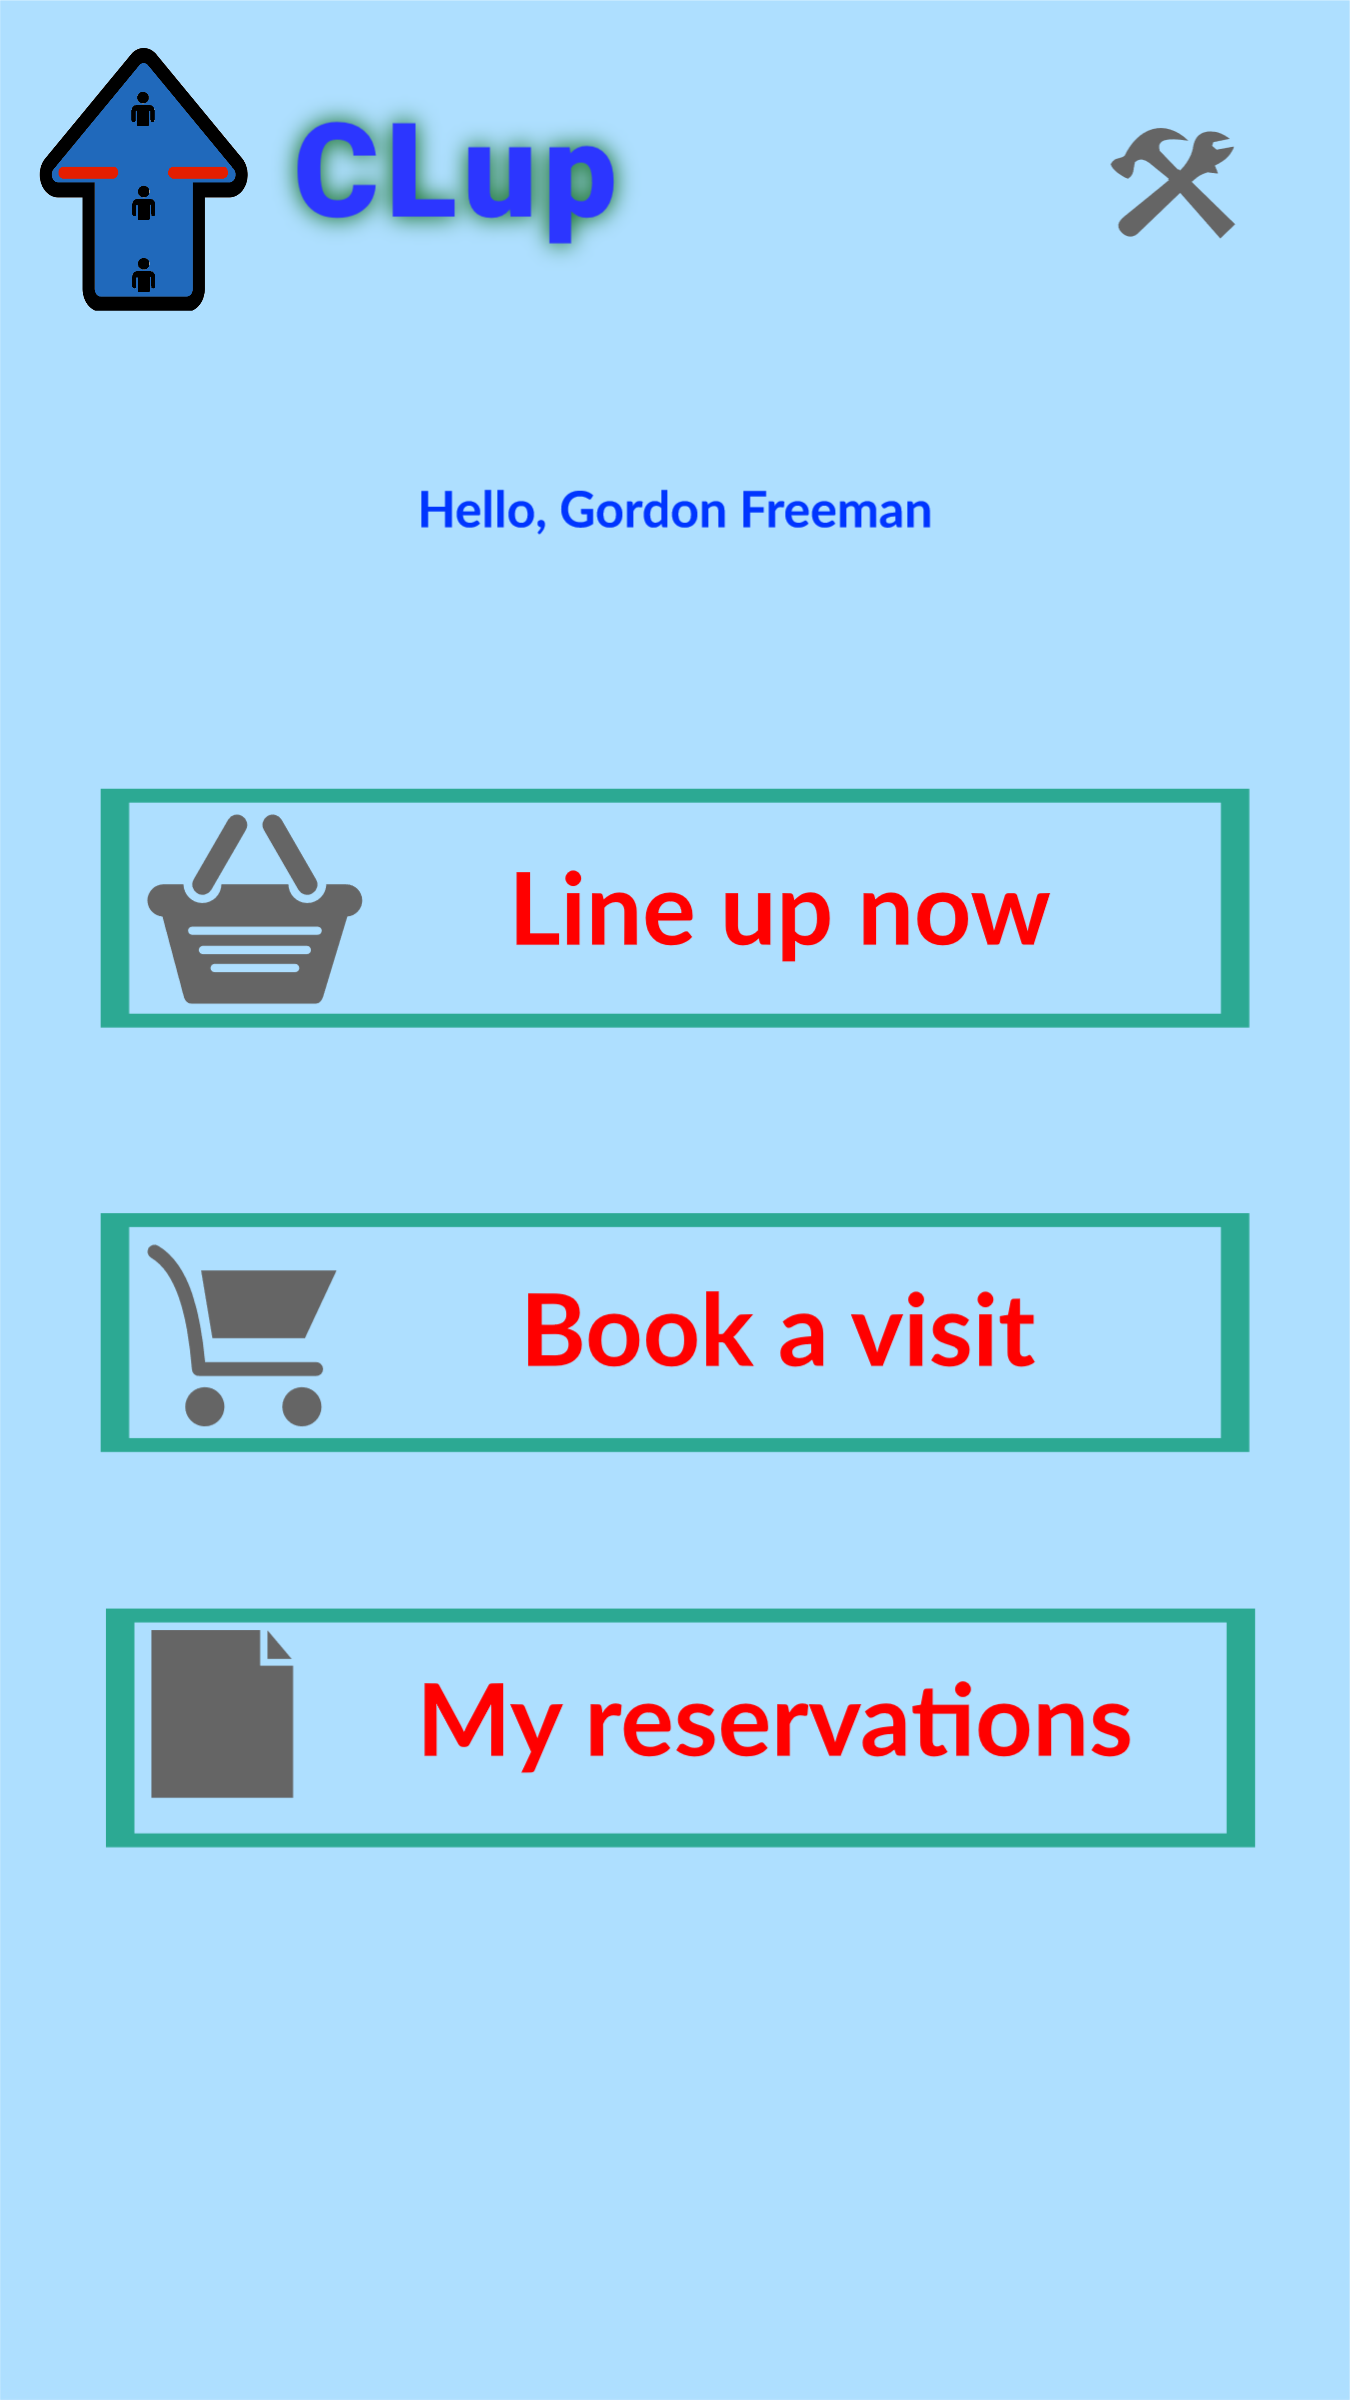
\includegraphics[scale=0.1]{Images/MainMenuCustomer.png}
	\qquad
	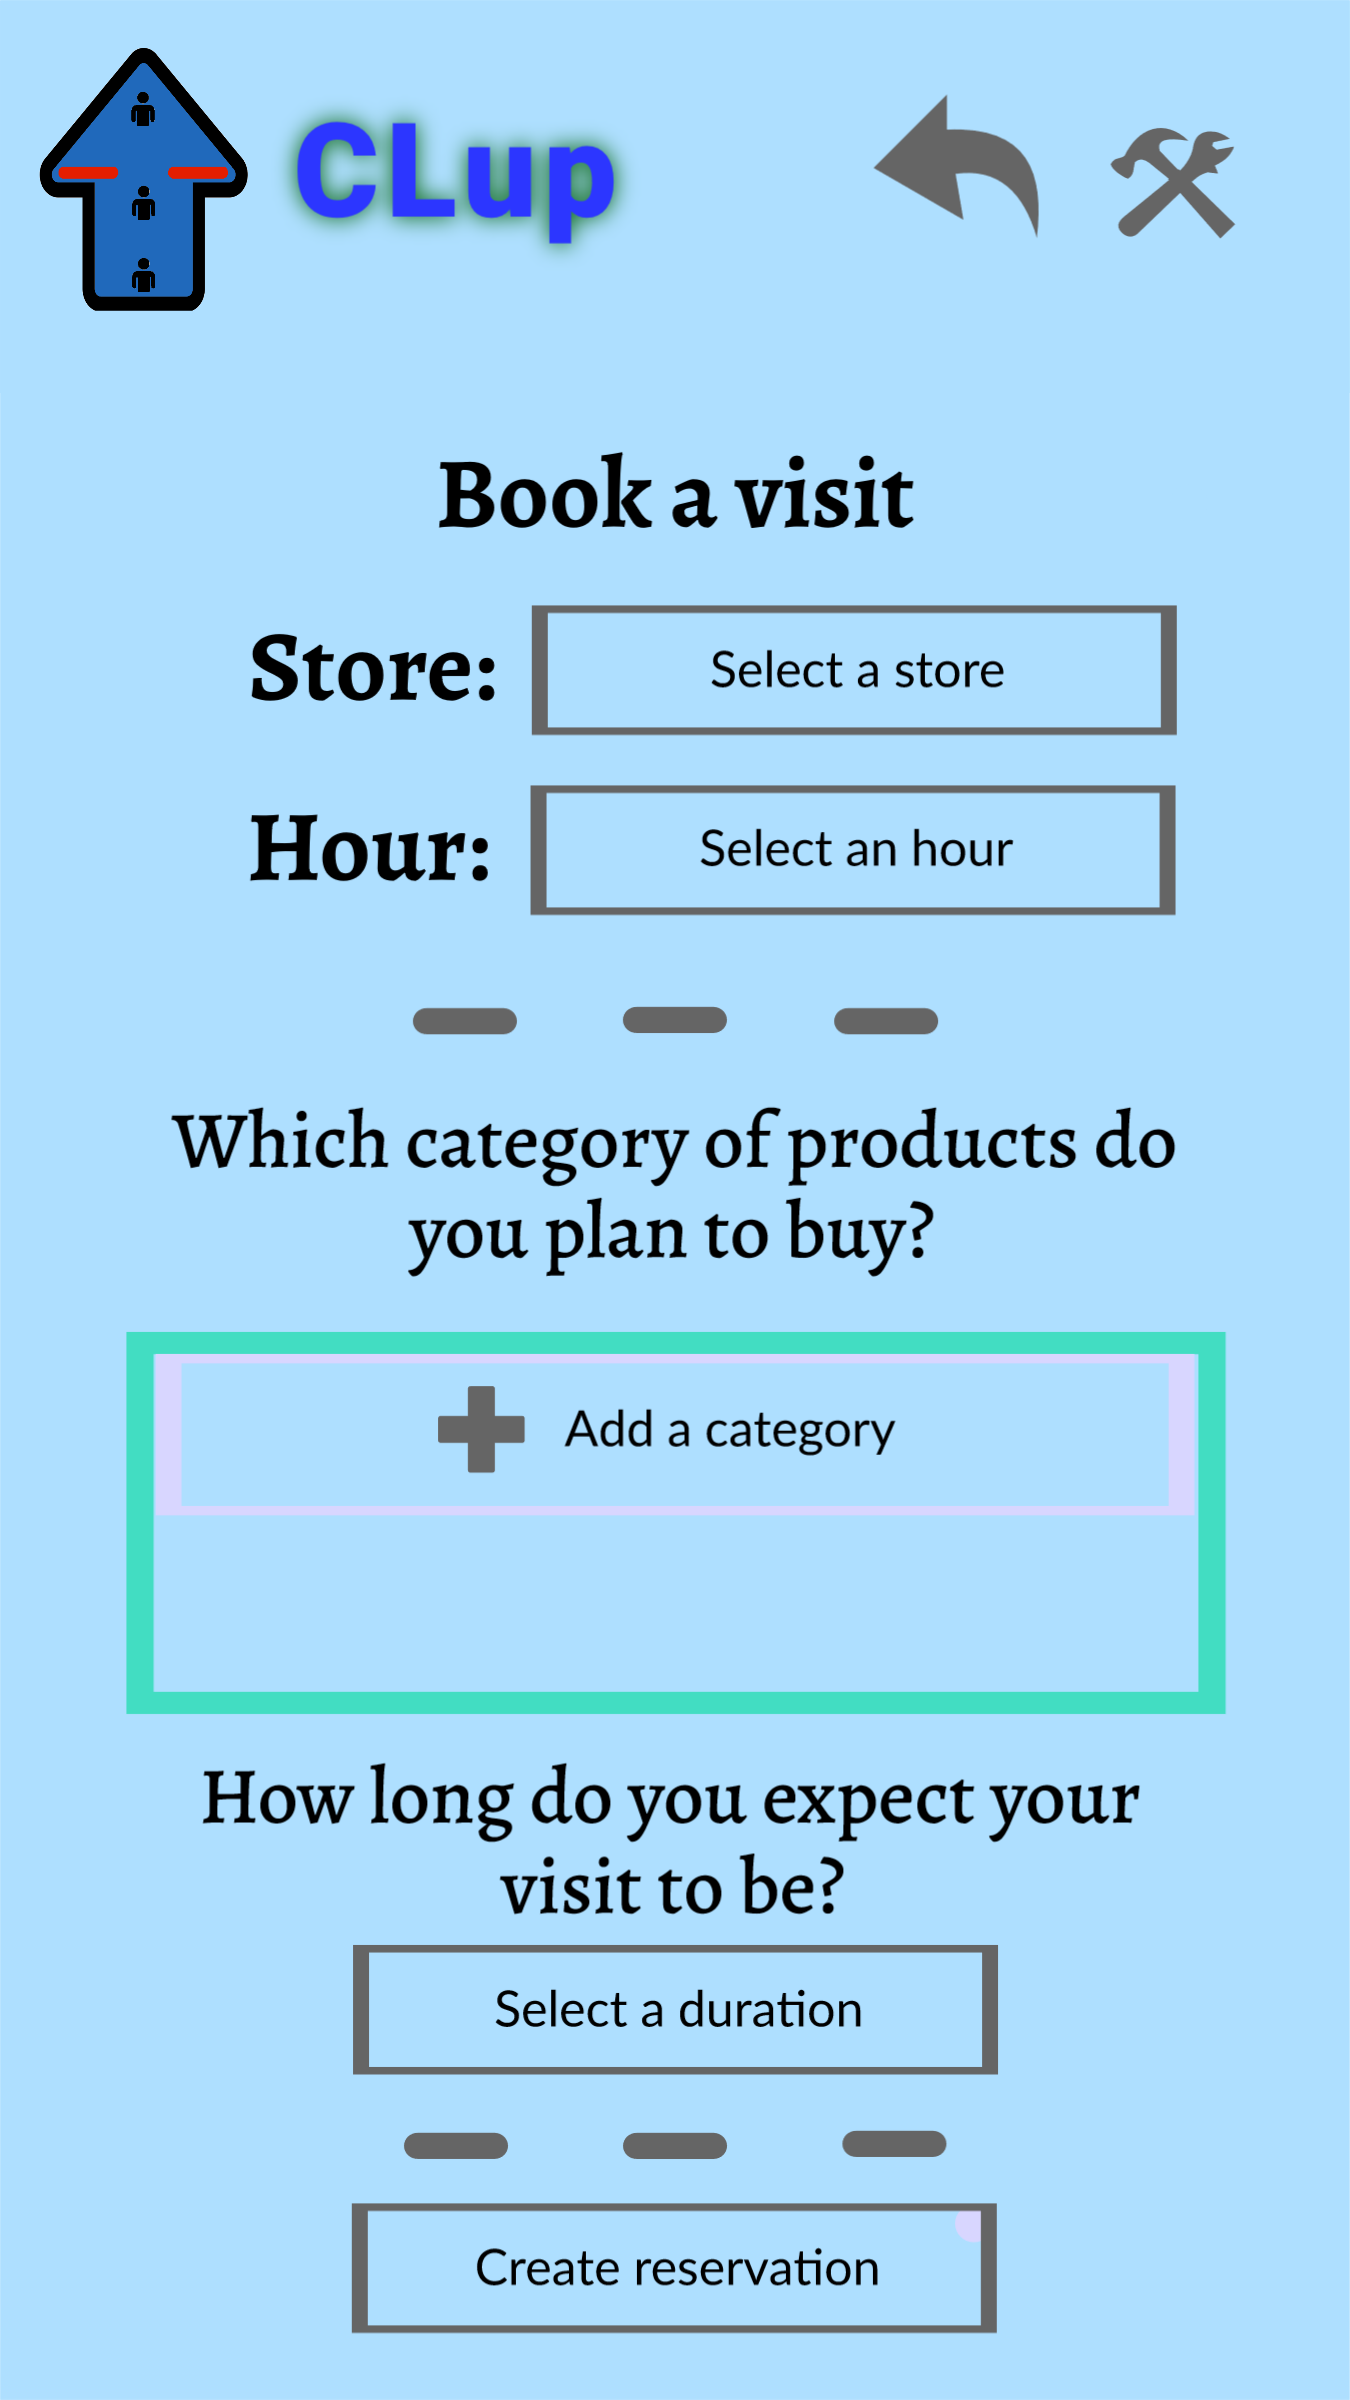
\includegraphics[scale=0.1]{Images/BookAVisit.png}
	\qquad
	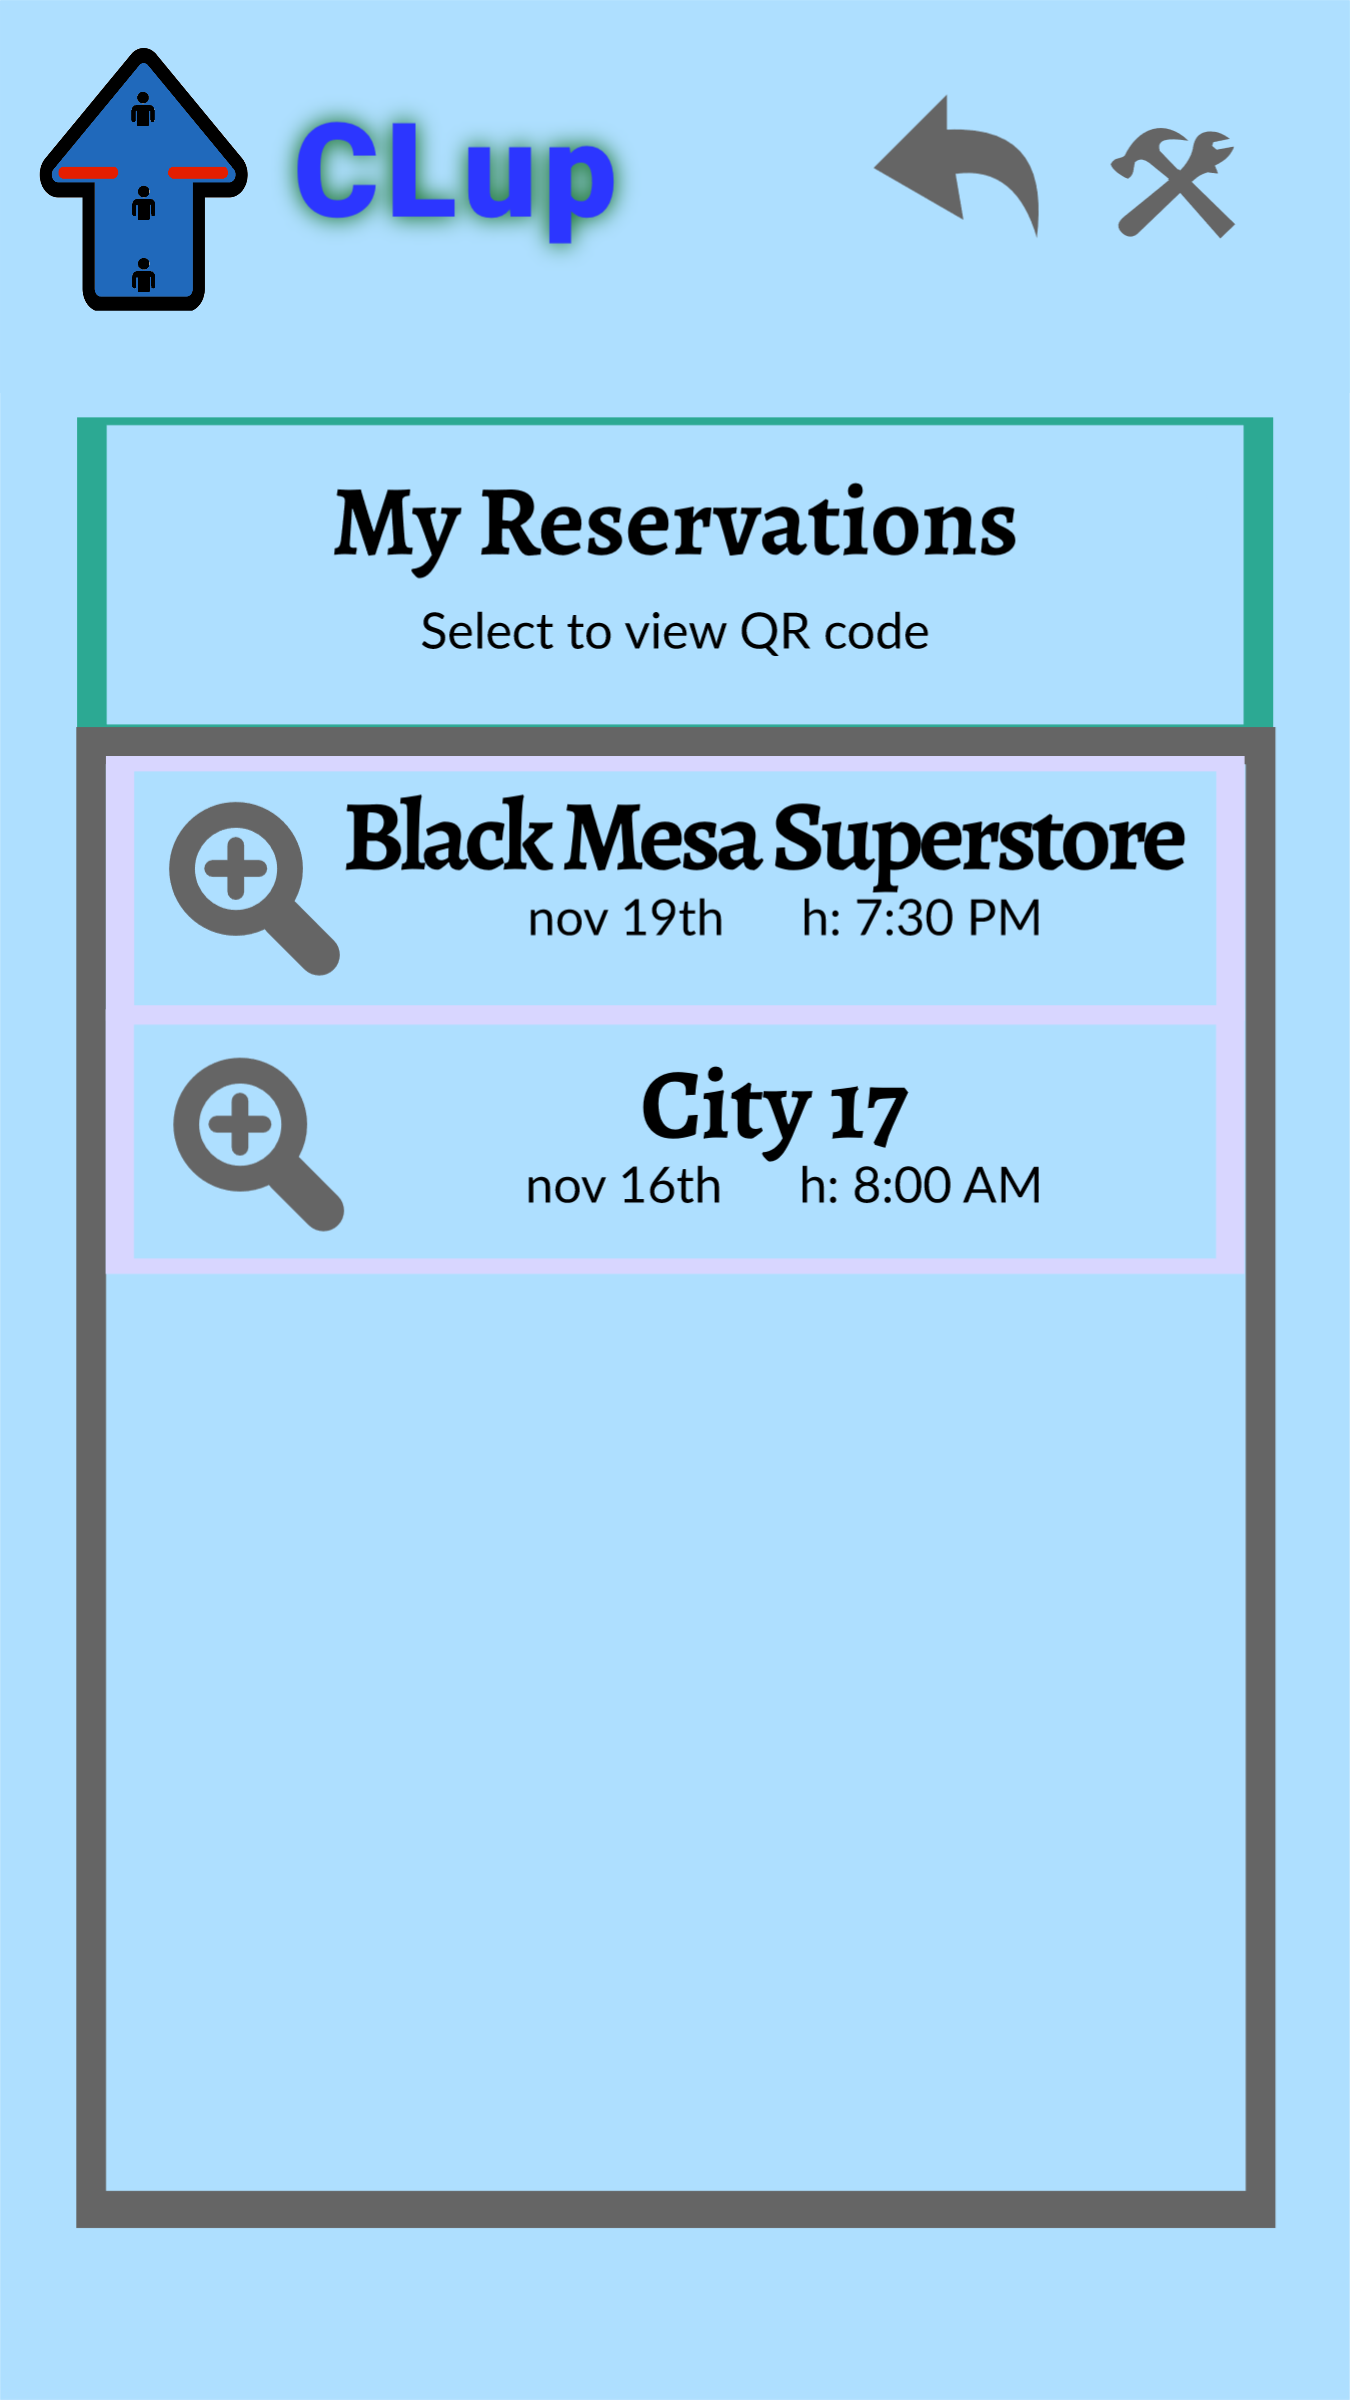
\includegraphics[scale=0.1]{Images/ShowReservations.png}
	\item {\bfseries Store owners}\\
	The store owner is presented with a main menu from which he/she can:
		\begin{itemize}
		\item register a store to the system
		\item delete a store from the system
		\item view and edit occupation for currently registered stores
	\end{itemize}
	\begin{figure}[!htb]
		\centering
		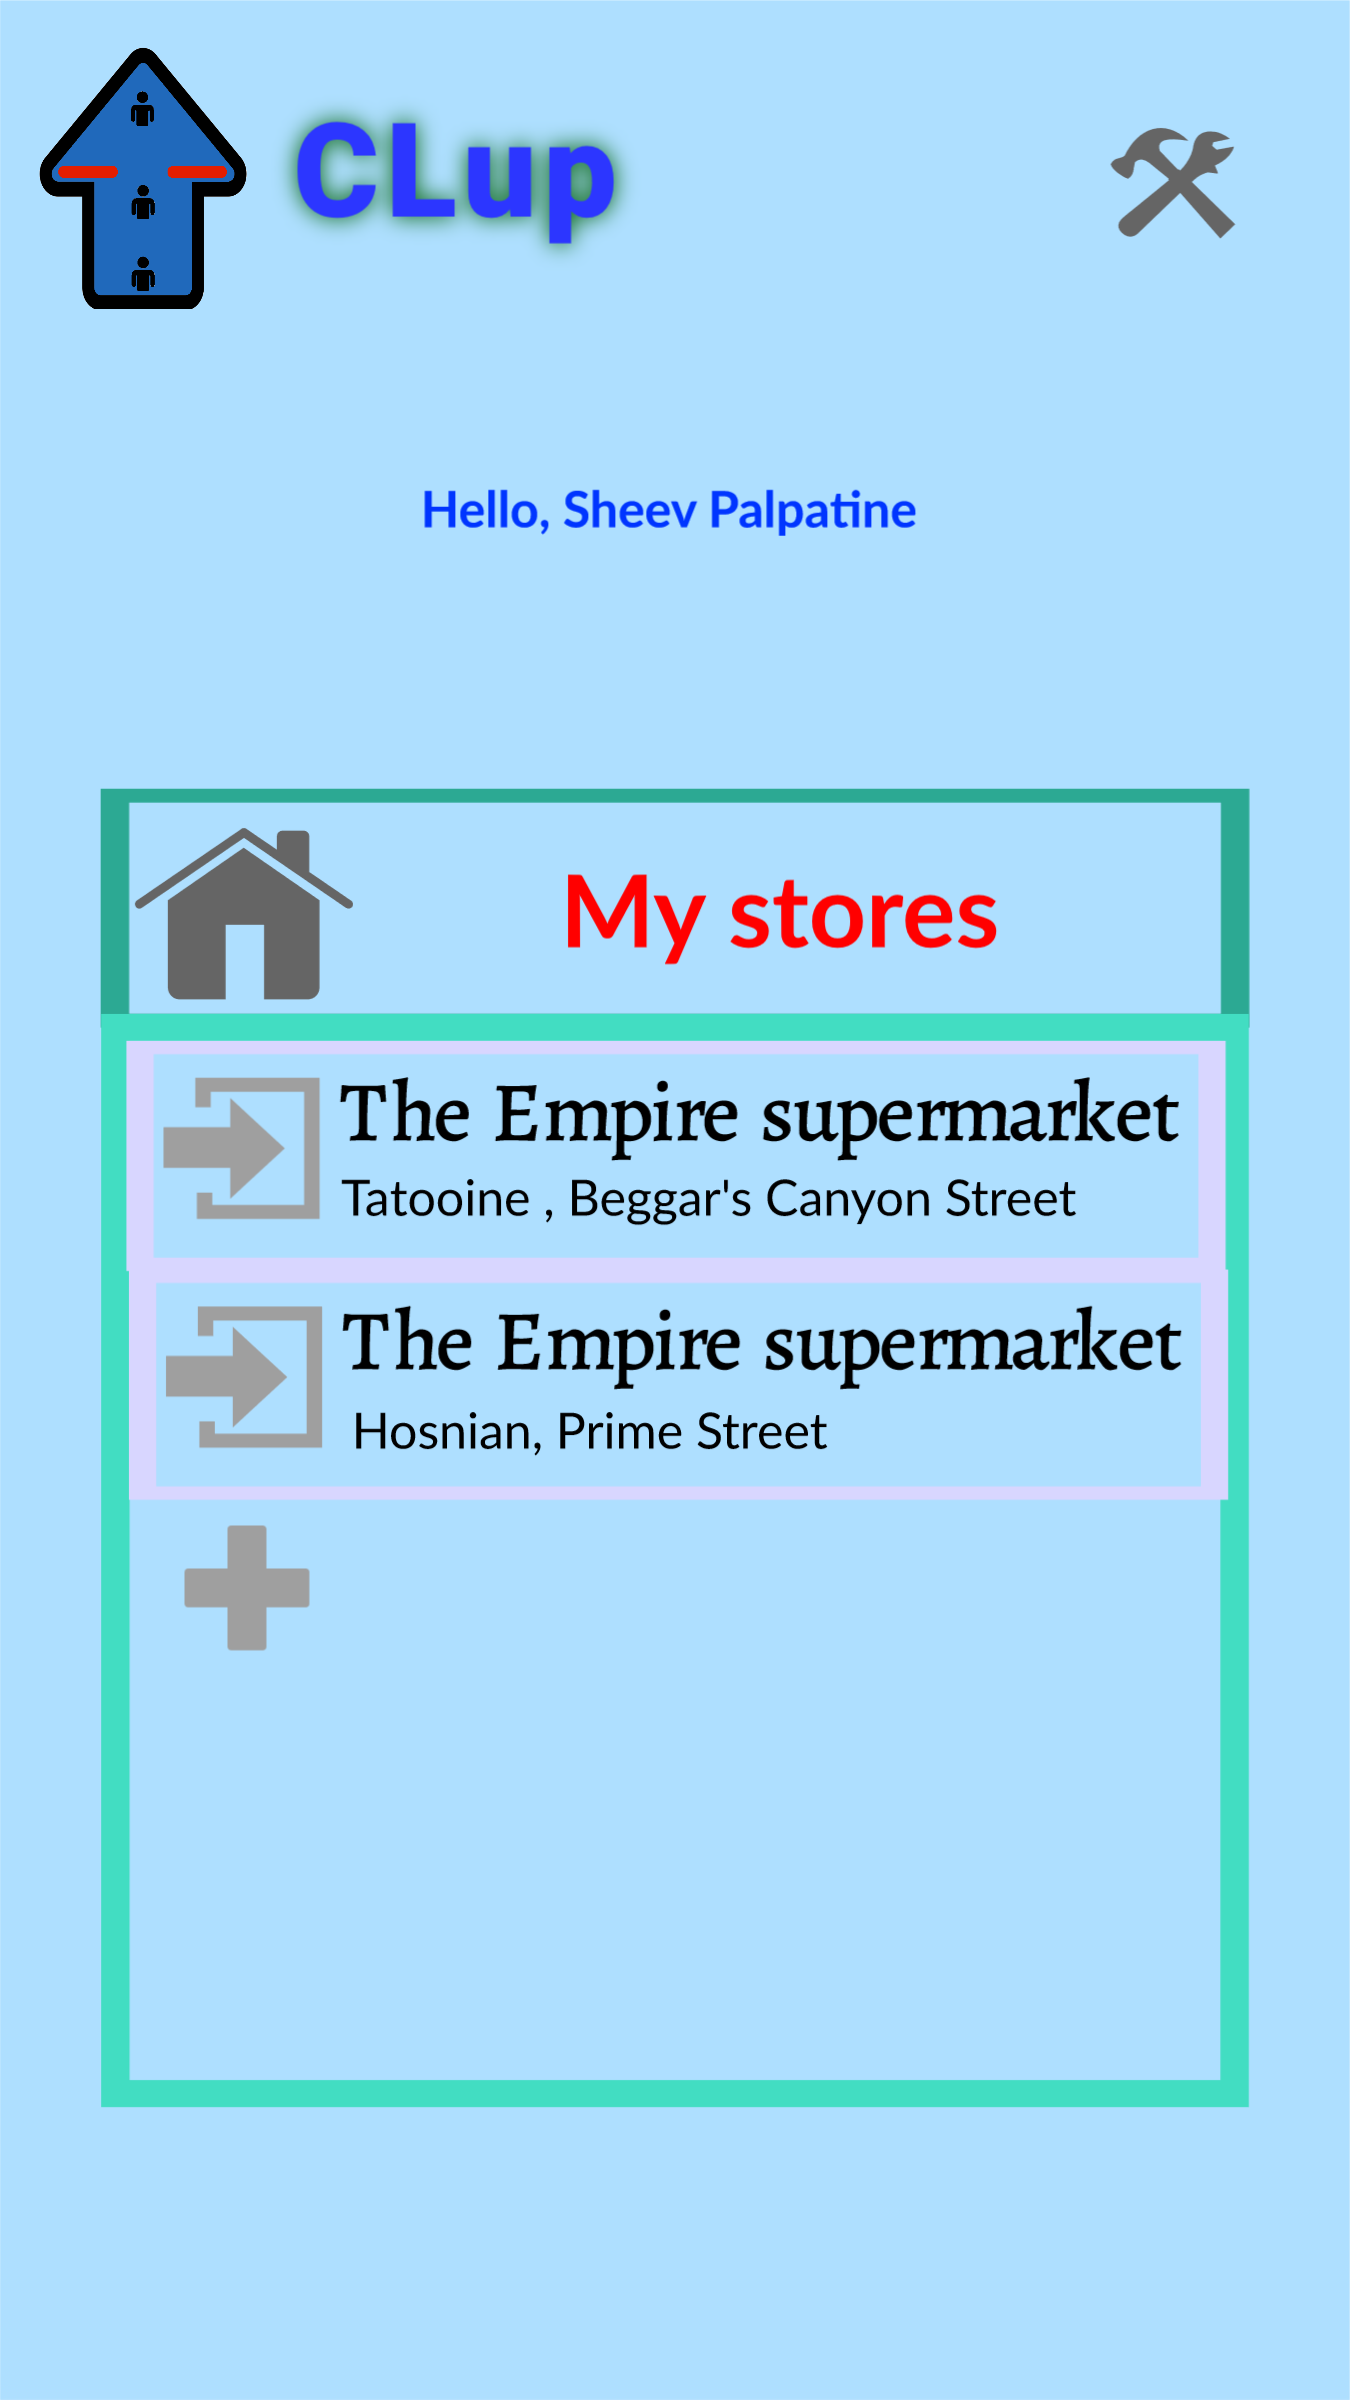
\includegraphics[scale=0.1]{Images/MainMenuOwner.png}
		\qquad \qquad
		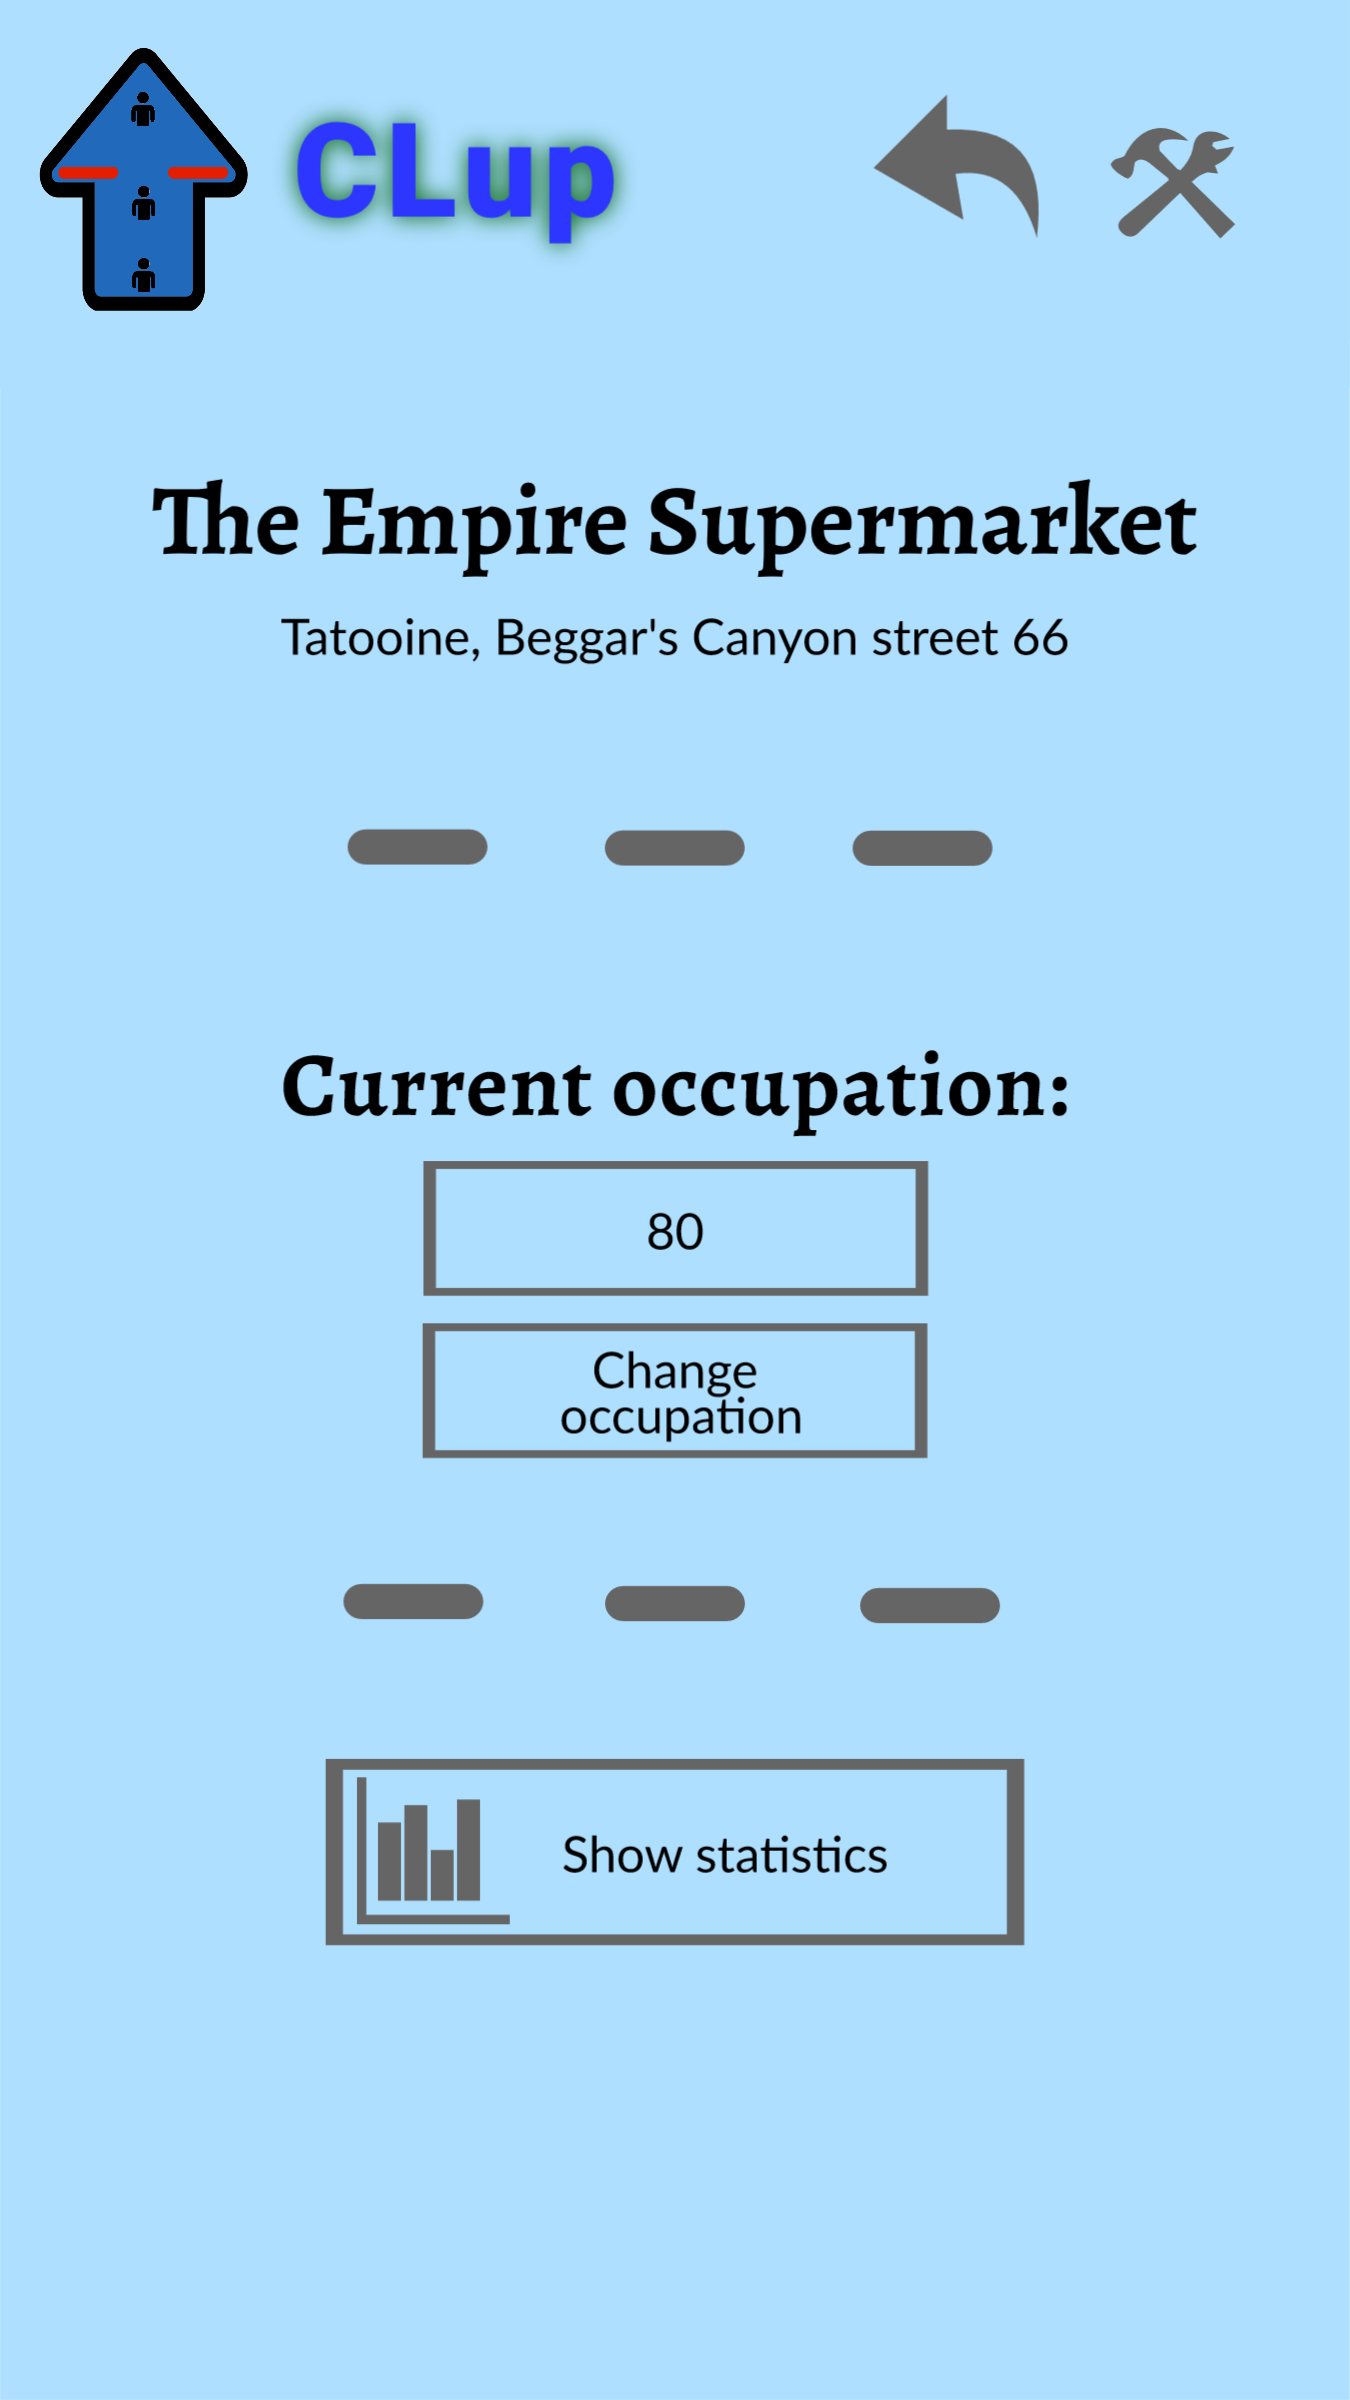
\includegraphics[scale=0.1]{Images/ModifyOccupation.png}
	\end{figure}
	\newpage
\end{itemize}
\subsubsection{Hardware interfaces}
The S2B requires the following hardware interfaces:
\begin{enumerate}
	\item {\bfseries Computer or smartphone}\\
	Users will need a computer or a smartphone to access the system's services which are provided via an application (only for smartphone owners) and a web application. Only users with an application will be able to receive notifications that alert them when it is time for them to depart and reach the store.
	\item {\bfseries Turnstiles}\\
	Turnstiles allow authorized customers to enter or exit the store by providing a means of identification. (i.e. QR, NFC)
	\item {\bfseries Ticket printer}\\
	The ticket printers located outside stores allows potential customers to queue up on premise provided that they identify themselves (e.g. social security card).
	\item \textbf{Monitor}\\
	A monitor located outside stores allows customers that queue up on premise to know when it is time for them to access the store.
\end{enumerate}

\subsubsection{Software interfaces}
The system uses a public API to locate the customer and provide him/her with notifications about the time he will need to depart to reach the store.

\subsubsection{Communication interfaces}
Customers can access the system through a working internet connection.

\subsection{Functional requirements}
\subsubsection{List of requirements}
\begin{enumerate}[label=R\arabic*]
	\item Turnstiles unlock if and only if activated by authorized customers.
	\item The number of customers in each department of the store never exceeds the occupation set by the owner.
	\item The monitor outside the store displays the number of the last authorized customer.
	\item The system allows customers and store owners to register and log in.
	\item The system validates the authenticity of the identifying information provided.
	\item The system allows customers to search for a store among those registered by their owners.
	\item Registered customers can send a reservation request to the system.
	\item Non registered customers with an identifying document can request reservations through the printer.
	\item Registered customers that book a visit can specify estimated visit duration.
	\item Registered customers that book a visit can specify desired product categories.
	\item The system provides customers with a QR code to enter the store once authorized.
	\item The system uses gathered data to build statistics.
	\item Registered customers with a smartphone are alerted when their turn is near.

	\item Registered customers can delete a pending or authorized reservation.
	\item Authorized reservations expire if they do not become current in a certain time window (specified by store owner)
	\item Registered customers must specify desired means of transport while requesting a reservation.
	\item Reservations are authorized according to a FIFO policy
\end{enumerate}
\subsubsection{Mapping on requirements}
\begin{tabular}{ | m{3cm} | m{5cm} | m{9cm} | }
	\hline
	G1 & D1, D2, D5, D6, D8, D9 & R1, R2, R4, R5, R6, R7, R11, R16, R17\\
	\hline
	G2 & D1, D2, D3, D4, D5, D6 & R1, R2, R3, R5, R8, R11, R17\\
	\hline
	G3 & D1, D2, D3, D4, D5, D6, D8, D9 & R1, R2, R3, R4, R5, R6, R7, R9, R10, R11, R16, R17\\
	\hline
	G4 & D1, D2, D5, D8, D9 & R1, R2 \\
	\hline
	G5 & D8, D9 & R9, R12, R14, R15\\
	\hline
	G6 & D4, D7, D8, D9 & R3, R13\\
	\hline
\end{tabular}
\newpage
Here we remind the goals for ease of use:
\begin{enumerate}[label=G\arabic*]
	\item CLup should allow customers to queue up remotely
	\item CLup should allow customers to queue up on premise
	\item CLup should allow customers to book future visits to stores
	\item CLup should allow store owners to regulate the maximum number of customers in their stores
	\item CLup should provide the customer with a reasonably precise estimate of waiting time
	\item CLup should alert the customers when it is time to get to the shop taking into account travel time
\end{enumerate}

Here we remind the domain assumptions for ease of use:
\begin{enumerate}[label=D\arabic*]
	\item The stores have QR activated turnstiles.
	\item Turnstiles let one and only one person in each time they unlock.
	\item Outside stores is a social security card activated ticket printer.
	\item Outside stores there is a monitor.
	\item There is no way for a customer to enter a store except from entrance and exit.
	\item Each customer has either a telephone number or an identification document.
	\item When provided, user location has maximum error of 5 meters.
	\item To register to the S2B users must have either a smartphone or a computer.
	\item To register and use the S2B users must have an internet connection.
\end{enumerate}
\subsubsection{Use case diagram}
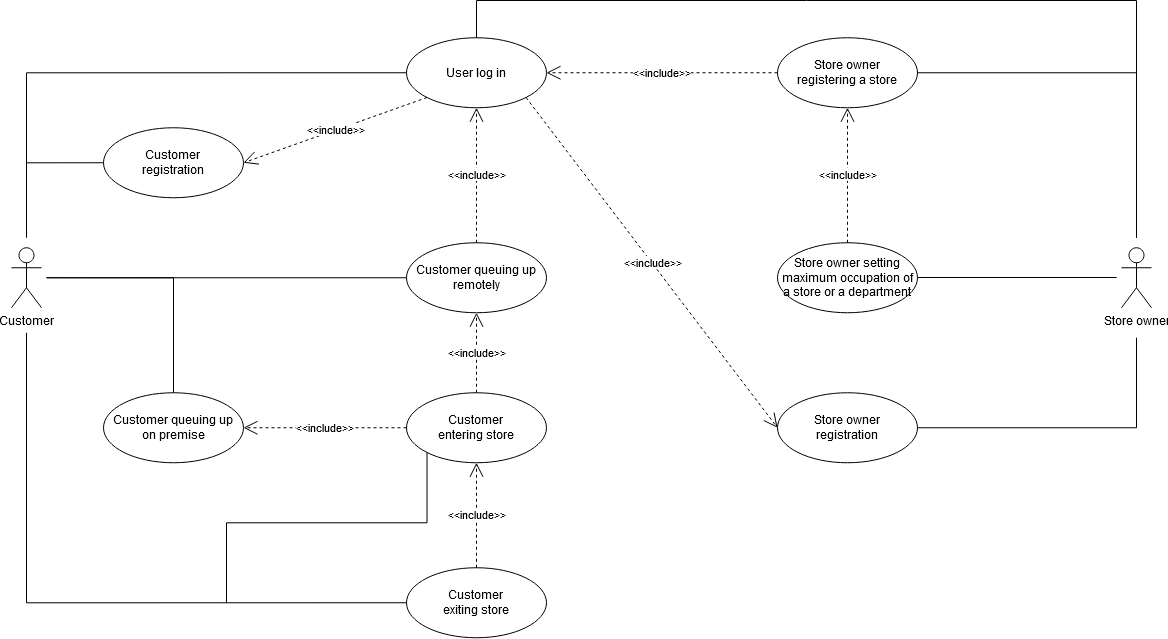
\includegraphics[scale=0.4]{Images/Use Case Diagram.png}
\newpage
\subsubsection{Use cases}
\paragraph{Customer registration}
\begin{flushleft}
	\begin{tabular} { | m{3cm} | m{10cm} | }
		\hline
		Name & Customer registration\\
		\hline
		Actors & Customer\\
		\hline
		Entry condition & Customer has opened the smartphone application or the web app on his computer but has not logged in\\
		\hline
		Event flow & \begin{enumerate}
			\item a registration menu is provided to the customer
			\item from such menu the customer selects the option to sign up as customer
			\item the customer is then prompted to insert identifying information
			\item the customer inserts requested information
			\item the system validates provided information
			\item the system confirms the registration of the customer and saves information provided
		\end{enumerate}\\
		\hline
		Exit conditions & Customer has registered to the system\\
		\hline
		Exceptions & \begin{enumerate}
			\item a customer with same identifying information already exists
			\item validation of identifying information is not successful
			\item the customer decides to cancel the registration
		\end{enumerate}
		If one of the first two events described above occur, the application will alert the customer and provide him with the possibility to retry or go back to the initial menu.\newline If event 3 occurs the customer is redirected to the main page.\\
		\hline
	\end{tabular}
\end{flushleft}
\newpage
\paragraph{Store owner registration}
\begin{flushleft}
	\begin{tabular} { | m{3cm} | m{10cm} | }
		\hline
		Name & Store owner registration\\
		\hline
		Actors & Store owner\\
		\hline
		Entry condition & Store owner has opened the smartphone application or the web app on his computer but has not logged in\\
		\hline
		Event flow & \begin{enumerate}
			\item a registration menu is provided to the store owner
			\item from such menu the store owner selects the option to sign up as store owner
			\item the store owner is then prompted to insert identifying information
			\item the store owner inserts requested information
			\item the system validates provided information
			\item the system confirms the registration of the store owner and saves information provided
		\end{enumerate}\\
		\hline
		Exit conditions & Store owner has registered to the system\\
		\hline
		Exceptions & \begin{enumerate}
			\item a store owner with same identifying information already exists
			\item validation of identifying information is not successful
			\item the store owner decides to cancel the registration
		\end{enumerate}
		If one of the first two events described above occur, the application will alert the store owner and provide him with the possibility to retry or go back to the initial menu.\newline If event 3 occurs the store owner is redirected to the main page.\\
		\hline
	\end{tabular}
\end{flushleft}

\paragraph{User logs in}
\begin{flushleft}
	\begin{tabular} { | m{3cm} | m{10cm} | }
		\hline
		Name & User logs in\\
		\hline
		Actors & Customer or store owner\\
		\hline
		Entry condition & The user has opened the application on his device, and has already registered to the system\\
		\hline
		Event flow & \begin{enumerate}
            \item User chooses to log in from the welcome menu
            \item User identifies him/herself with created credentials
		\end{enumerate}\\
		\hline
		Exit conditions & User is logged in\\
		\hline
		Exceptions & \begin{enumerate}
			\item User credentials are invalid
		\end{enumerate}
		If the event described above occurs, the application will alert the user and allows him to retry\\
		\hline
	\end{tabular}
\end{flushleft}
\newpage
\paragraph{Customer queuing up remotely}
\begin{flushleft}
	\begin{tabular} { | m{3cm} | m{10cm} | }
		\hline
		Name & Customer queuing up remotely\\
		\hline
		Actors & Customer\\
		\hline
		Entry condition & Customer has logged in on the smartphone application or the web app on his computer\\
		\hline
		Event flow & \begin{enumerate}
			\item customer selects to queue up from main menu
			\begin{itemize}
				\item with an immediate reservation
				\item with a future reservation (and optionally inserts desired categories of item he/she intends to buy and how much time he/she intends to spend at the store)
			\end{itemize}
			\item customer selects a store from the list of stores registered to the system
			\item customer specify  whether he is going to reach the store by car or on foot
			\item customer submits reservation request
		\end{enumerate}\\
		\hline
		Exit conditions & Customer reservation is confirmed\\
		\hline
		Exceptions & \begin{enumerate}
			\item customer decides to cancel the reservation
			\item customer requests immediate reservaiton but store is closed at that time
		\end{enumerate}
		If one of the events described above occur, the application will alert the customer and go back to the initial menu\\
		\hline
	\end{tabular}
\end{flushleft}
\newpage
\paragraph{Customer queuing up on premise}
\begin{flushleft}
	\begin{tabular} { | m{3cm} | m{10cm} | }
		\hline
		Name & Customer queuing on premise\\
		\hline
		Actors & Customer\\
		\hline
		Entry condition & Customer has reached the store ticket printer\\
		\hline
		Event flow & \begin{enumerate}
			\item customer selects the option to queue up from main menu of the ticket printer
			\item customer provides the ticket printer with a means of identification (e.g. social security card)
		\end{enumerate}\\
		\hline
		Exit conditions & Customer reservation is confirmed and a ticket is printed containing the following information:
		\begin{itemize}
			\item how much time he needs to wait before being able to enter the store
			\item a progressive number that will allow him to know when his/her turn is
		\end{itemize}\\
		\hline
		Exceptions & \begin{enumerate}
			\item customer decides to cancel the reservation
		\end{enumerate}
		If one of the events described above occur, the application will alert the customer and go back to the initial menu\\
		\hline
	\end{tabular}
\end{flushleft}

\paragraph{Customer entering store}
\begin{flushleft}
	\begin{tabular} { | m{3cm} | m{10cm} | }
		\hline
		Name & Customer entering store\\
		\hline
		Actors & Customer\\
		\hline
		Entry condition & Customer has logged in on the smartphone application and is at the entrance of a store or has printed authorization from the web app\\
		\hline
		Event flow &
		If the customer has not printed the reservation ticket he must use his smartphone:
		\begin{enumerate}
			\item customer selects the option to show existing reservations from main menu of the phone app 
			\item customer selects an existing reservation and if authorized (i.e. it is his turn to enter the store) he/she is given the means to identify him/herself (e.g. display QR or activate NFC)
		\end{enumerate}
		Then the customer identifies him/herself at the turnstiles\\
		\hline
		Exit conditions & Customer enters the store\\
		\hline
		Exceptions & \begin{enumerate}
			\item customer is not authorized to enter the store
		\end{enumerate}
		If the event described above occurs, the turnstiles will not let the customer in\\
		\hline
	\end{tabular}
\end{flushleft}
\newpage
\paragraph{Customer exiting store}
\begin{flushleft}
	\begin{tabular} { | m{3cm} | m{10cm} | }
		\hline
		Name & Customer exiting store\\
		\hline
		Actors & Customer\\
		\hline
		Entry condition & Customer has logged in on the smartphone application and is in a store\\
		\hline
		Event flow &
		If the customer has not printed the reservation ticket he must use his smartphone:
		\begin{enumerate}
			\item customer selects the option to show existing reservations from main menu
			\item customer selects an existing reservation and if authorized (i.e. it is his turn to enter the store) he/she is given the means to identify him/herself (e.g. display QR or activate NFC)
		\end{enumerate}
	    Customer identifies him/herself at the turnstiles\\
		\hline
		Exit conditions & Customer exits the store\\
		\hline
		Exceptions & \\
		\hline
	\end{tabular}
\end{flushleft}

\paragraph{Store owner registering a store}
\begin{flushleft}
	\begin{tabular} { | m{3cm} | m{10cm} | }
		\hline
		Name & Store owner registering a store\\
		\hline
		Actors & Store owner\\
		\hline
		Entry condition & Store owner has logged in on the smartphone application or the web app on his computer\\
		\hline
		Event flow & \begin{enumerate}
			\item store owner selects the option register a store from main menu
			\item store owner inserts necessary information and sets up equipment (i.e. connect printer, monitor and turnstiles to the system)
			\item store owner submits store registration request
		\end{enumerate}\\
		\hline
		Exit conditions & Store registration is confirmed\\
		\hline
		Exceptions & \begin{enumerate}
			\item information is missing or incorrect
			\item equipment is not working properly			\item store owner decides to cancel the store registration
		\end{enumerate}
		If one of the events described above occur, the application will alert the store owner and provide him with the possibility to retry or go back to the initial menu\\
		\hline
	\end{tabular}
\end{flushleft}
\newpage
\paragraph{Store owner setting maximum occupation of a store or a department}
\begin{flushleft}
	\begin{tabular} { | m{3cm} | m{10cm} | }
		\hline
		Name & Store owner setting maximum occupation of a store or a department\\
		\hline
		Actors & Store owner\\
		\hline
		Entry condition & Store owner has logged in on the smartphone application or the web app on his computer\\
		\hline
		Event flow & \begin{enumerate}
			\item store owner selects one of his stores from the list reachable form the main menu
			\item store owner views current occupation of each department of his store, and current occupation threshold
			\item sets the new desired occupation threshold for a department or for the whole store
		\end{enumerate}\\
		\hline
		Exit conditions & The new occupation threshold is set\\
		\hline
		Exceptions & \begin{enumerate}
			\item the threshold value is inadequate
		\end{enumerate}
		If the event described above occurs, the application will alert the store owner and provide him with the possibility to retry or go back to the initial menu\\
		\hline
	\end{tabular}
\end{flushleft}
\paragraph{Customer is alerted}
\begin{flushleft}
	\begin{tabular} { | m{3cm} | m{10cm} | }
		\hline
		Name & Customer is alerted\\
		\hline
		Actors & Customer\\
		\hline
		Entry condition & Customer is logged into his smartphone application and the time he/she needs to wait becomes less or equal to the time he/she needs to reach the store\\
		\hline
		Event flow & \begin{enumerate}
			\item The system sends a notification to the smartphone of the customer
		\end{enumerate}\\
		\hline
		Exit conditions & Customer is notified\\
		\hline
		Exceptions & \begin{enumerate}
			\item the threshold value is inadequate
		\end{enumerate}
		If the event described above occurs, the application will alert the store owner and provide him with the possibility to retry or go back to the initial menu\\
		\hline
	\end{tabular}
\end{flushleft}
\newpage
\subsubsection{Sequence diagrams}
\paragraph{Customer registration}
\begin{flushleft}
	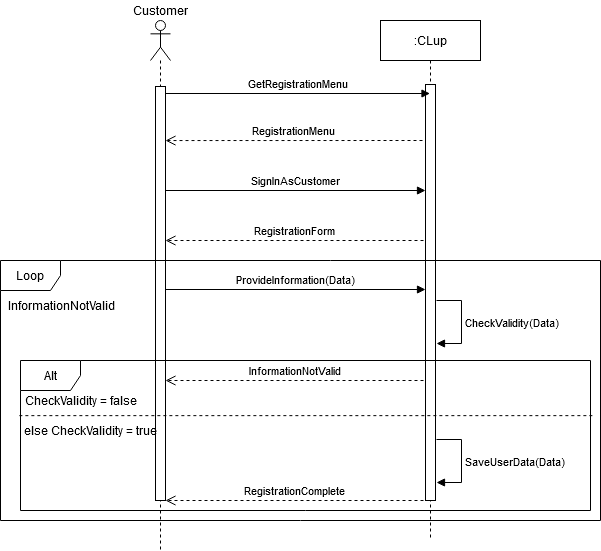
\includegraphics[scale=0.5]{Images/UseCase1Diagram.png}
\end{flushleft}
\paragraph{Store owner registration}
\begin{flushleft}
	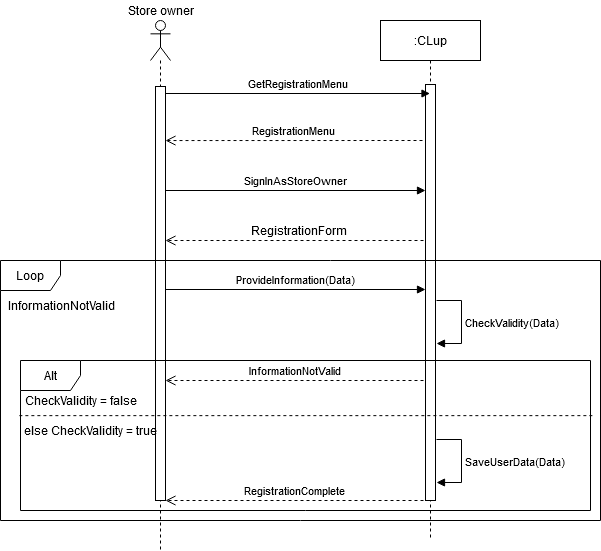
\includegraphics[scale=0.5]{Images/UseCase2Diagram.png}
\end{flushleft}
\newpage
\paragraph{User logs in}
\begin{flushleft}
	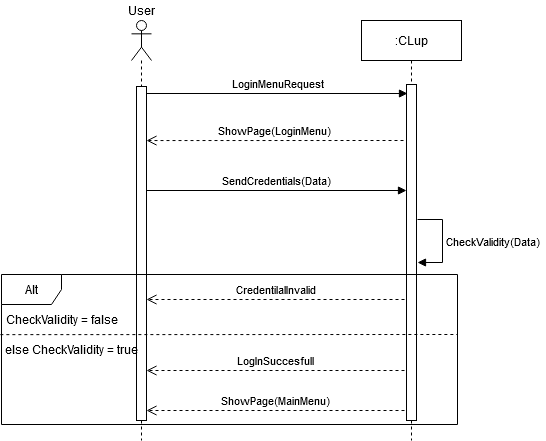
\includegraphics[scale=0.5]{Images/UseCase3Diagram.png}
\end{flushleft}
\paragraph{Customer queuing up remotely}
\begin{flushleft}
	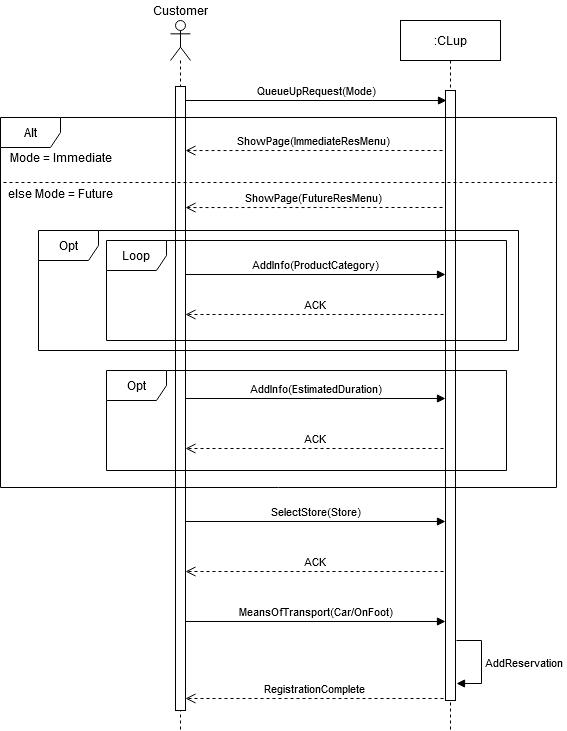
\includegraphics[scale=0.5]{Images/UseCase4Diagram.png}
\end{flushleft}
\newpage
\paragraph{Customer queuing up on premise}
\begin{flushleft}
	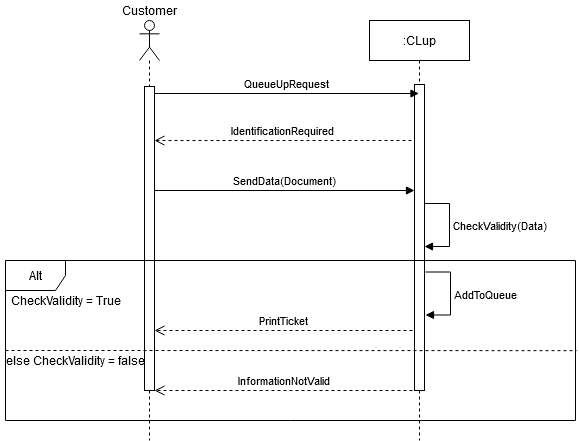
\includegraphics[scale=0.5]{Images/UseCase5Diagram.png}
\end{flushleft}
\paragraph{Customer entering and exiting store}
\begin{flushleft}
	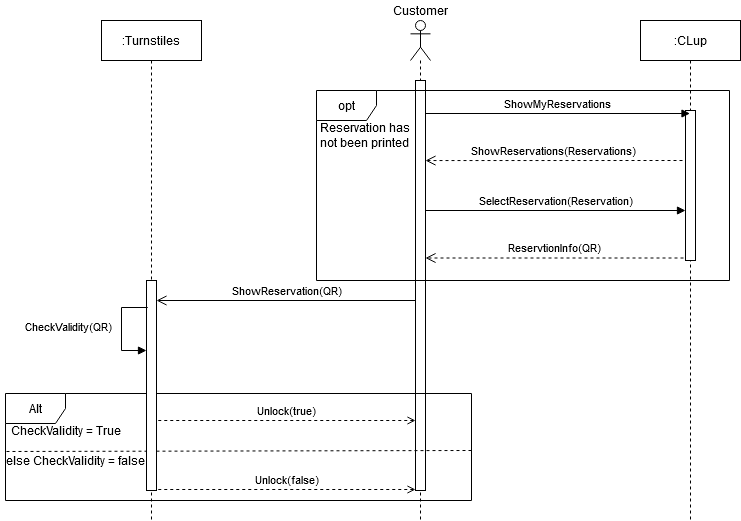
\includegraphics[scale=0.5]{Images/UseCase6-7Diagram.png}
\end{flushleft}
\newpage
\paragraph{Store owner registering a store}
\begin{flushleft}
	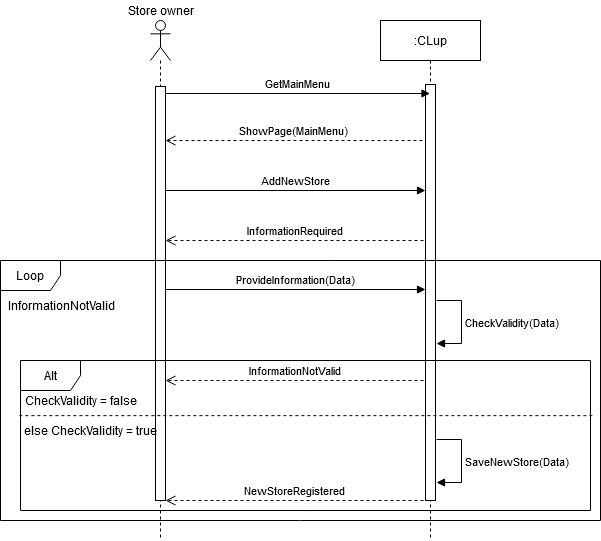
\includegraphics[scale=0.5]{Images/UseCase8Diagram.png}
\end{flushleft}
\paragraph{Store owner setting maximum occupation of a store or a department}
\begin{flushleft}
	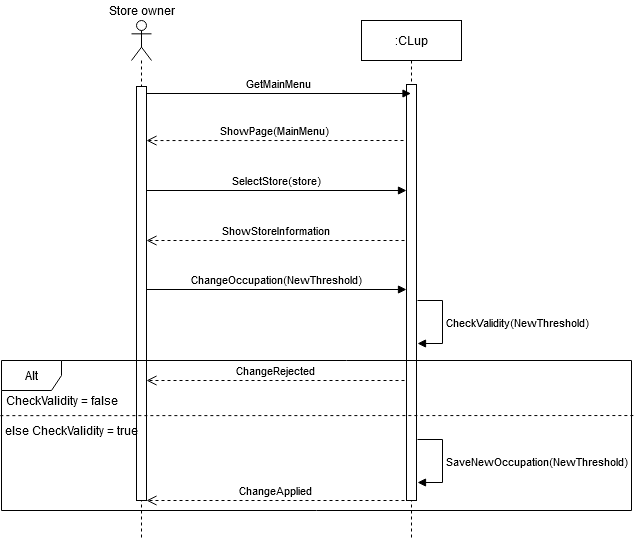
\includegraphics[scale=0.5]{Images/UseCase9Diagram.png}
\end{flushleft}
\newpage
\paragraph{Customer is alerted}
\begin{flushleft}
	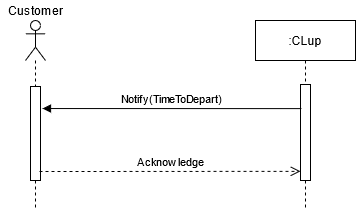
\includegraphics[scale=0.5]{Images/UseCase10Diagram.png}
\end{flushleft}

\subsection{Performance Requirements}
The system cannot guarantee that a customer can enter a store at a precise time unless it requires users to exit after a maximum time (which it doesn't).
The system guarantees that if
\begin{itemize}
	\item the customer uses a smartphone
	\item the customer never disconnects from the internet and GPS
	\item the customer specified the correct means of transport when creating the reservation
\end{itemize}
 he/she will be alerted when he needs to depart to reach a store (in order not to be late) with a delay of at most 10 seconds.
\subsection{Design Constraints}
\subsubsection{Standards compliance}
The code should follow the requirements contained in this document, and be thoroughly commented.
\subsubsection{Hardware limitations}
The software the customer uses requires either:
\begin{itemize}
	\item a smartphone to use the smart application
	\item a computer to use the web application and a home printer to print reservation
\end{itemize}
The software the store owner uses requires:
\begin{itemize}
	\item turnstiles activated by QR
	\item reservation printer activated by social security card
	\item monitor to alert on premise customers when it is their turn
\end{itemize}
\subsubsection{Any other constraint}
Customers cannot have more than five active reservation requests for different stores and more than two for the same store on the same day to avoid fake reservations.
\subsection{Software System Attributes}
\subsubsection{Reliability}
The system must have an appropriate infrastructure with a full backup system located in an separate office distant at least 100km (nuclear fallout radius). Adequate personnel will guarantee recovery time to substitute faulty hardware.
\subsubsection{Availability}
The system should be up for 99.9\% of the time (0.365 MTTR). Its temporary downtime does not cause emergency situations, but the system is an essential service: it should be possible to buy food every day. The system is fully automated. The users are alerted about system downtime with a delay of at most 10 minutes. The users are alerted that the system is up again with a delay of at most 10 minutes.
\subsubsection{Security}
The location of customers is sensitive information and therefore is never stored. Customers and store owners provide identifying information during registration: the databases containing such information must be protected against internal and external attacks. Communication between central system and users is encrypted.
\subsubsection{Maintainability}
The system is easy to maintain: its code is thoroughly commented and modular. Appropriate design patterns are exploited.
\subsubsection{Portability}
The smartphone application runs under Android and iOS. The web application runs under Android, iOS, Windows, MacOS.

%------------------------------------------------------------------------------------------------------------------------------------------------
\clearpage
{\color{Blue}{\section{Formal Analysis Using Alloy}}}
\label{sect:alloy}
\subsection{Alloy Code}
This section is dedicated to the Alloy model of the CLup  software, included all the functions of the application and their most important constraints.\\
In the model are represented the two categories of users: the store owners and the customers. Each store owner owns a set of stores, and each customer opens a set of reservations. Those reservations can be of three types: immediate, on premise and future. Every reservation refers to a store, has an estimated time for the customer who opened it to reach the store, a time for that customer to wait before he/she is able to enter, a value representing in which moment the reservation has been created, and a boolean value, representing whether the customer has already been alerted (he/she must depart to reach the store). Moreover each reservation can be in one of 4 states:
\begin{itemize}
	\item PENDING: reservation has been requested but customer cannot yet access the store
	\item AUTHORIZED: customer can access the store for a time window
	\item CURRENT: customer has accessed the store and has not exited yet
	\item EXPIRED: customer has exited the store or the time window to enter the store ended or the reservation was deleted
\end{itemize}
Finally a future reservation keeps track of entry time.

We apply some constraints to the model so that it can represent the application domain of our S2B.\\
First, customers are queued up following a First In First Out policy. We ensure that the parameters in the reservations are meaningful with respect to the state of the reservation itself, e.g. a customer is alerted when the time remaining before it is his/her turn is less or equal than the time for him/her to reach the store. For every store we check that the current occupation is equal to the number of customer inside the store and that this value never exceeds the maximum occupation of that store.

\VerbatimInput{alloy.als}
\newpage
\subsection{Scenarios}
Those are some instances of the Alloy model based on the predicates above.
\begin{flushleft}
	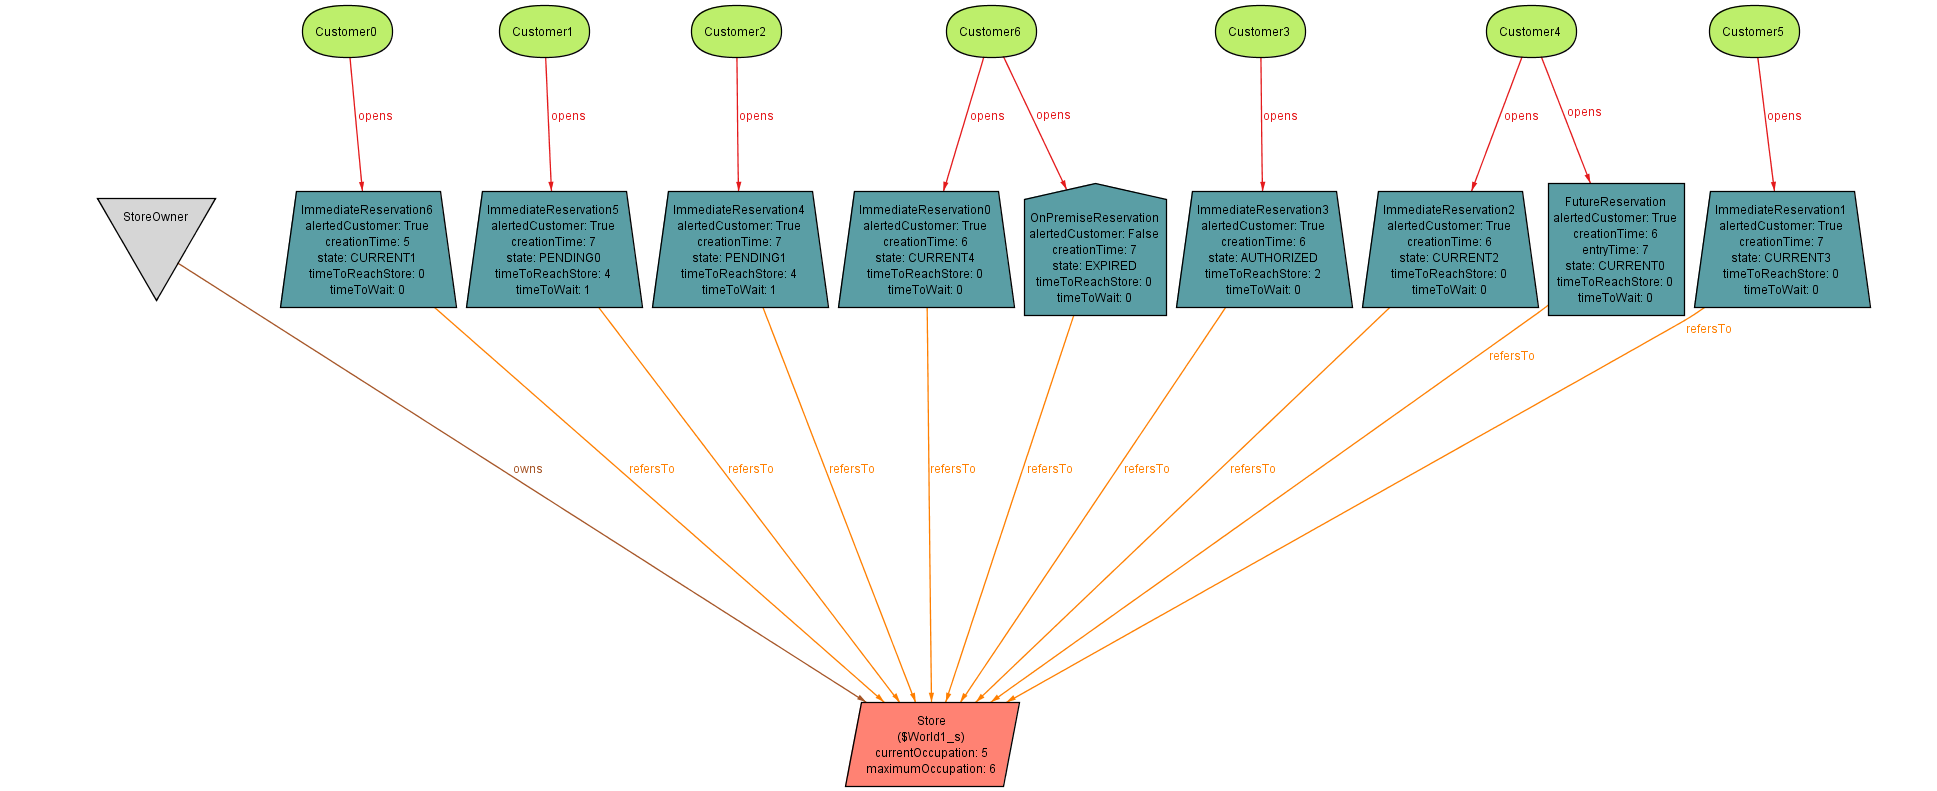
\includegraphics[scale=0.25]{Images/Alloy_World1.png}
\end{flushleft}
The first scenario shows a store with a current occupation of 5, which represents the actual number of current reservations, and we observe that it is still less than the maximum occupation.\\\\

\begin{flushleft}
	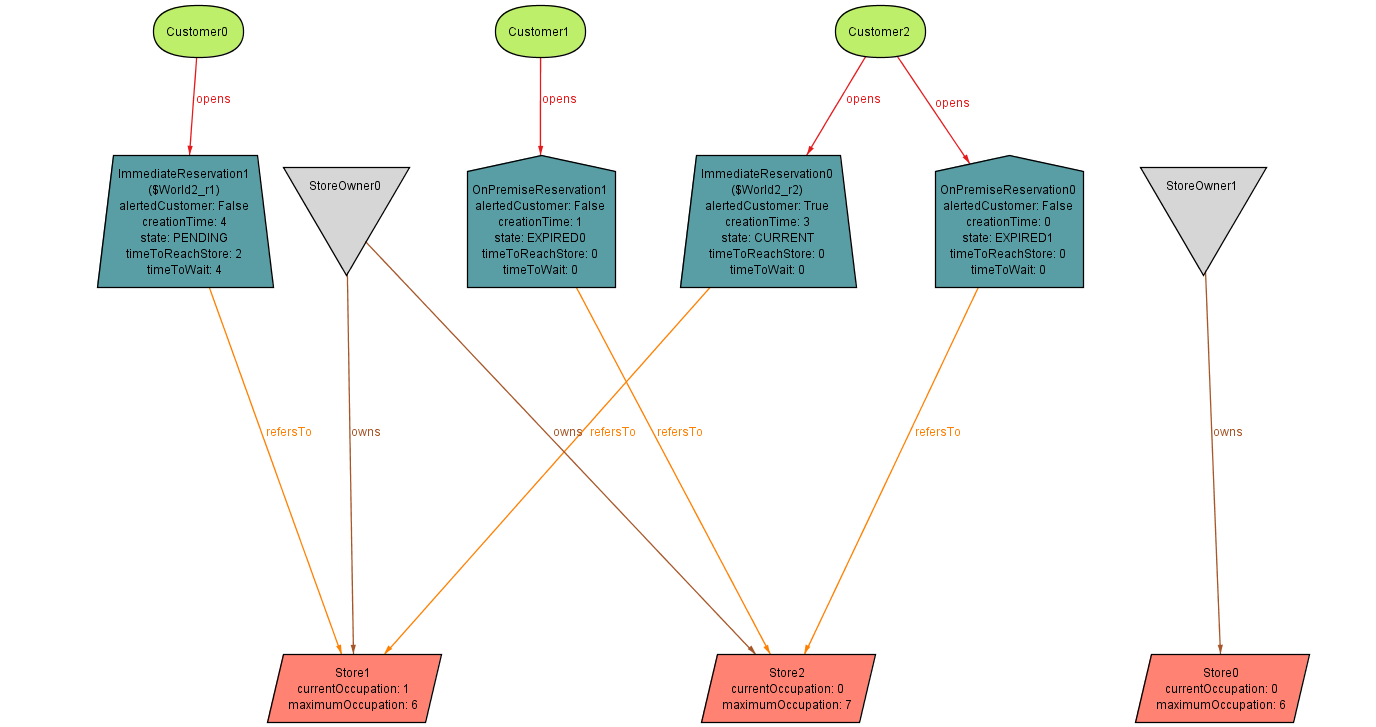
\includegraphics[scale=0.3]{Images/Alloy_World2.png}
\end{flushleft}
In the second scenario there are two immediate reservations r1 and r2 for the same store. r1 has been created after r2, so r2 has less time to wait with respect to r1.\\
Moreover the customer that opened r2 has been alerted because his time to wait is less or equal than the time for him to reach the store, while for r1 this property doesn't hold, so the customer has not been alerted.\\\\

\begin{flushleft}
	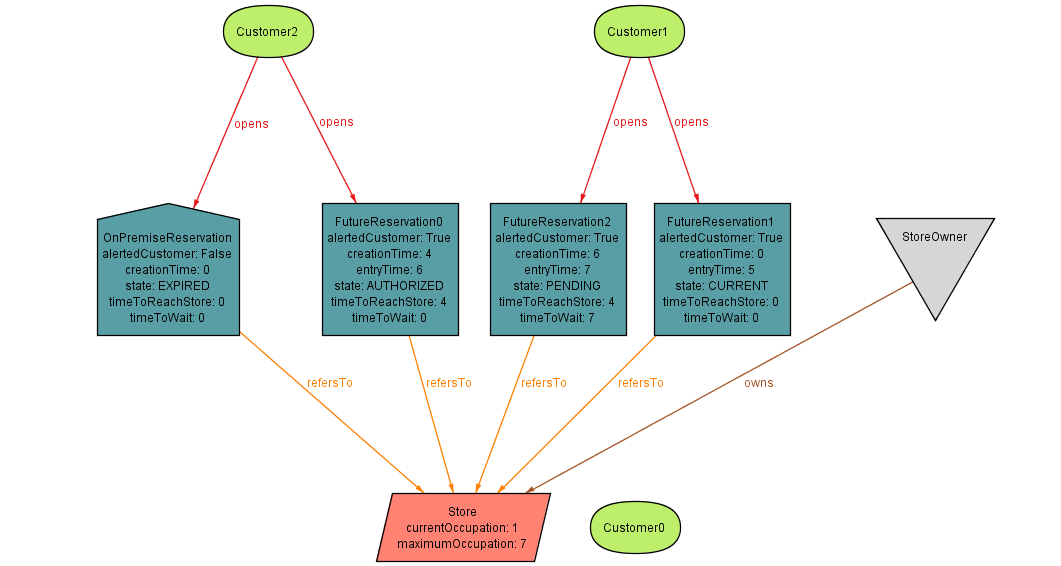
\includegraphics[scale=0.4]{Images/Alloy_World3.png}
\end{flushleft}
In the third scenario there is a customer which has not opened any reservation yet.\\
Customer 1 has booked two reservations and they have different entry time.\\\\

\begin{flushleft}
	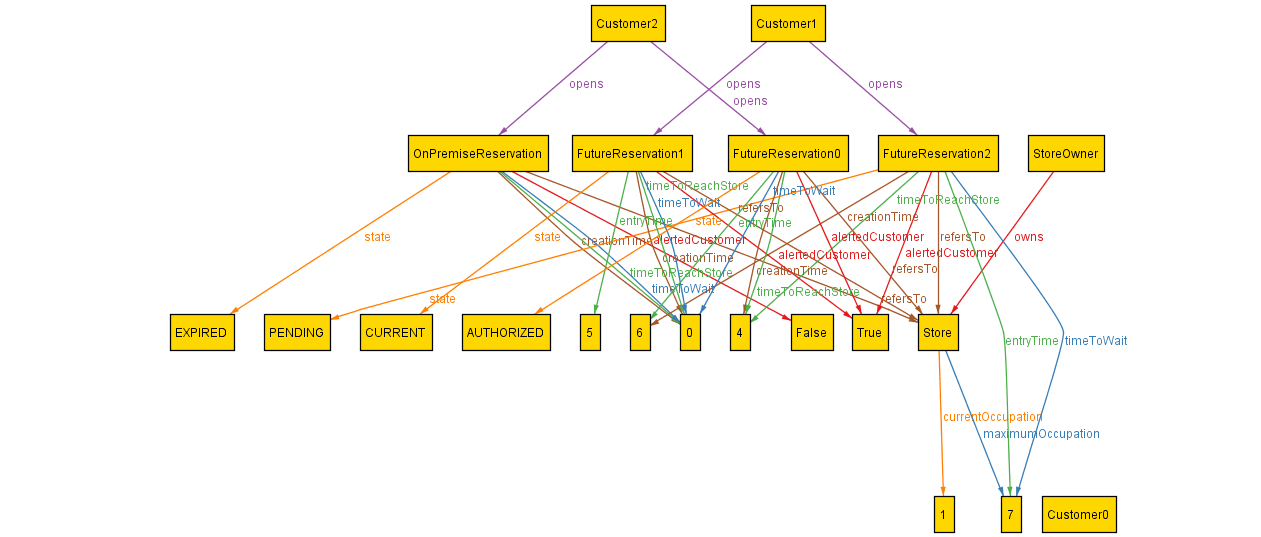
\includegraphics[scale=0.4]{Images/Alloy_World3_ugly.png}
\end{flushleft}
We used a theme in the diagrams above to make them more readable; without the theme the third diagram would look like this.





%------------------------------------------------------------------------------------------------------------------------------------------------
\clearpage
{\color{Blue}{\section{Effort Spent}}}
\label{sect:effort}
\subsection{Simone Abelli}
\begin{tabular} { | m{5cm} | m{1cm} | }
	\hline
	Introduction & 3.5\\
	\hline
	UML class diagram & 4\\
	\hline
	Product perspective & 3\\
	\hline
	State charts, External interface requirements & 4.5\\
	\hline
	User interfaces & 4.5\\
	\hline
	Requirements & 6.5\\
	\hline
	Sequence diagrams & 3.5\\
	\hline
	Scenarios & 0.5\\
	\hline
	Alloy & 7\\
	\hline
\end{tabular}

\subsection{Stefano Azzone}
\begin{tabular} { | m{5cm} | m{1cm} | }
	\hline
	Introduction & 3\\
	\hline
	UML class diagram & 3\\
	\hline
	Product perspective & 3\\
	\hline
	Product functions, user characteristics, domain assumptions & 2.5\\
	\hline
	State charts, External interface requirements & 3\\
	\hline
	Use cases & 3.5\\
	\hline
	Alloy & 11.5\\
	\hline
	Requirements & 6.5\\
	\hline
	Performance Requirements, Design constraints, Software system attributes, first two scenarios & 1\\
	\hline
\end{tabular}


%------------------------------------------------------------------------------------------------------------------------------------------------
\clearpage
\addcontentsline{toc}{section}{References}
\bibliographystyle{plain}
\bibliography{main}
%------------------------------------------------------------------------------------------------------------------------------------------------




\end{document}
